% Manuscript v7 | 2026-09-28 | Final local v3 data including own VP benchmark.
% Tables between DATA markers are regenerated by tools/build_results.py.
\documentclass{article}
\PassOptionsToPackage{numbers,compress}{natbib}
\usepackage[final,main]{neurips_2026}
\usepackage[utf8]{inputenc}
\usepackage[T1]{fontenc}
\usepackage{amsmath,amssymb,booktabs,graphicx,microtype,url}
\usepackage{algorithm,algpseudocode}
\usepackage{xcolor,tikz}
\usetikzlibrary{arrows.meta,positioning}
\usepackage{hyperref}
\hypersetup{hidelinks,pdftitle={BDG: Batch-Dispersion Guidance for Property-Band Generation},pdfsubject={Manuscript v7, 28 September 2026}}
\newcommand{\Fbar}{\bar F}
\newcommand{\Vb}{V_b}
\newcommand{\weff}{w_{\mathrm{eff}}}
\newcommand{\IB}{\mathrm{IB}}
\newcommand{\sg}{\operatorname{stopgrad}}
\title{BDG: Batch-Dispersion Guidance for\\Property-Band Generation}
\author{Bobo Li, Henry Huang, Idea Idehpour\\
Department of Computer and Information Science, University of Pennsylvania\\
\small Manuscript v7 \quad 28 September 2026}
\begin{document}
% MAIN_TEXT_START
\maketitle
\begin{abstract}
Property-targeted generation requires samples within a tolerance band while preserving sample quality. Standard gradient guidance couples movement toward a target with contraction of the generated property distribution. We introduce Batch-Dispersion Guidance (BDG), which adjusts the deviation coefficient using the discrepancy between predicted endpoint variance and a specified variance. The target-centering coefficient remains unchanged, and the update requires the same neural calls as plug-in guidance. We study QM9 molecules in Euclidean coordinates and DeepFlyBrain DNA sequences on a probability simplex. Our trained flow-matching model achieves higher molecular stability and validity than our variance-preserving diffusion model, supporting flow matching as the backbone for guidance and transfer. Across two molecular flow backbones and three properties, contracting BDG increases mean decoded band coverage by 0.45--1.52 percentage points over plug-in and reduces mean absolute target error in all six comparisons. These coverage gains remain below the protocol threshold, with greater seed variability on our flow model. A 612-cell gain--setpoint ablation demonstrates both narrowing and widening at fixed nominal strength. On DNA, contracting BDG increases CpG coverage by 4.82 and 16.83 points at strengths one and four, respectively. Hamming diversity remains nearly unchanged, while sequence-distribution mismatch increases. Comparisons with four recent guidance adaptations support BDG as a transferable means of adjusting property spread and band occupancy, with property-dependent quality trade-offs.
\end{abstract}

\section{Introduction}
Diffusion reverses corruption; flow matching learns a transport velocity \citep{karras2022elucidating,lipman2022flow}. Both generate structured samples from noise, but their quality and sampling cost require a matched comparison \citep{albergo2025stochastic}.

Gradient guidance couples target centering and spread \citep{chung2023dps,song2023lgd}. Motivated by batch interactions and moment constraints \citep{corso2024particle,mgd2026moment}, we ask whether endpoint-dispersion adjustment improves band coverage without excessive quality loss.

We study QM9 molecules and DeepFlyBrain DNA, selecting flow matching using a trained VP diffusion comparison. Our hypothesis is that BDG adjusts spread at fixed guidance strength and improves coverage across state spaces. Our contributions are summarized as follows.
\begin{itemize}
\item We compare trained FM and diffusion, with external references.
\item We derive BDG's plug-in reduction and repulsion condition.
\item We test gain and setpoint in 612 molecular ablation cells.
\item We compare recent guidance adaptations and quantify DNA transfer.
\end{itemize}

\section{Related Work}
\textbf{Continuous generation.} Flow matching fits path velocities; diffusion learns a reverse corruption process \citep{lipman2022flow,karras2022elucidating}. Stochastic interpolants connect these constructions \citep{albergo2025stochastic}.

\textbf{Dispersion and guidance.} Particle Guidance introduces batch interactions \citep{corso2024particle}; Moment Guided Diffusion imposes moment constraints \citep{mgd2026moment}; variance tilting favors feature spread \citep{vtd2026variance}. BDG contributes a scalar endpoint-variance residual inside property guidance, without their distributional guarantees.

\textbf{Molecules.} Equivariant diffusion and EquiFM model molecular geometry \citep{hoogeboom2022equivariant,song2023equifm}. We compare DPS-style plug-in, TMPD-inspired guidance, LGD-MC and TFG adaptations on common frozen backbones \citep{chung2023dps,boys2024tmpd,song2023lgd,ye2024tfg}.

\textbf{Sequences.} Dirichlet FM and Fisher Flow model simplex-valued sequences; MOG-DFM guides discrete biological sequences \citep{stark2024dirichlet,davis2024fisher,chen2025multi}. Our measured sequence comparators are ports of the guidance rules above, not reproductions of these three generators.

\section{Methods}
\subsection{Modalities, Data, and Preprocessing}\label{sec:data}
QM9 \citep{ramakrishnan2014qm9} uses centered coordinates and one-hot H/C/N/O/F types. Generator/guide $f_A$ and evaluator $f_B$ use disjoint halves of 51,527 molecules; validation/test contain 17,748/13,083. Targets are dipole $\mu$, polarizability $\alpha$, and HOMO--LUMO gap. DeepFlyBrain's 500-bp DNA occupies $(\Delta^3)^{500}$, a different state space, with 83,722/10,505/10,434 train/validation/test examples. Generators take no property input; molecules condition only on atom-count mask $M$ (Appendix~\ref{app:data}).

\subsection{Continuous Flow Matching Baseline}\label{sec:fm}
With Gaussian source $x_0$, data $x_1$ and uniform $t\in[0,1]$, we train
\begin{equation}
x_t=(1-t)x_0+tx_1,\qquad \mathcal L_{\rm FM}=\mathbb E\|v_\theta(x_t,t;M)-(x_1-x_0)\|_M^2.
\label{eq:fm}
\end{equation}
The 3.75M-parameter EGNN has eight layers of width 256. Training uses Adam, batch 256, initial rate $2\times10^{-4}$, cosine decay and EMA 0.9999. We evaluate epoch-1500 EMA weights with 100 Euler steps (Table~\ref{tab:training}).

\subsection{Diffusion Baseline}\label{sec:diff}
Our trained VP model uses the same representation and EGNN configuration. For corruption time $u$, $a(u)=\exp[-(0.1u+9.95u^2)/2]$ and $\sigma^2(u)=1-a^2(u)$:
\begin{equation}
x_u=a(u)x_1+\sigma(u)\epsilon,\qquad\mathcal L_{\rm VP}=\mathbb E\|\epsilon_\phi(x_u,u;M)-\epsilon\|_M^2.
\label{eq:vp}
\end{equation}
Sampling integrates $\mathrm dx/\mathrm du=-\frac12\beta(u)(x-\epsilon_\phi/\sigma)$ backward, with $\beta(u)=0.1+19.9u$, 100 steps and terminal denoising. We evaluate the selected epoch-1475 EMA checkpoint.

\subsection{Guided Generation}\label{sec:guidance}
The frozen guide evaluates $F_i=f_A(m_i)$ at $m_i=x_t^{(i)}+(1-t)v_\theta(x_t^{(i)},t;M)$. Let $s$ be the calibration-pool property standard deviation. For target $y$, plug-in guidance adds
\begin{equation}
G_i=\frac{y-F_i}{s^2}\nabla_{x_t^{(i)}}F_i,\qquad
C_i=\operatorname{clip}_{\|v_i\|}\!\left[w\frac{1-t}{\max(t,\varepsilon)}G_i\right].
\label{eq:plug}
\end{equation}
We apply $C_i$ for $t\ge0.5$, then mask and recenter molecular coordinates. The derivative includes the generator's endpoint Jacobian. All model weights stay frozen.

\subsection{Proposed Innovation: Batch-Dispersion Guidance}\label{sec:bdg}
For batch size $B$, set $\Fbar=B^{-1}\sum_iF_i$, $\Vb=(B-1)^{-1}\sum_i(F_i-\Fbar)^2$, and $\tau=\tau_m s$. BDG replaces $y-F_i$ by
\begin{equation}
\begin{aligned}
n_i&=(y-F_i)-\eta e(F_i-\Fbar)=(y-\Fbar)-\weff(F_i-\Fbar),\\
e&=(\Vb-\tau^2)/\tau^2,\qquad \weff=1+\eta e.
\end{aligned}\label{eq:bdg}
\end{equation}
The residual adjusts contraction around the batch mean while preserving the target-centering coefficient. Coefficients are detached before the pullback. \textbf{At $\eta=0$, BDG equals plug-in}; $\tau>0$ is required because $e$ divides by $\tau^2$. Negative $e$ weakens contraction; net repulsion requires $\weff<0$ and $\eta>1$. Gain and setpoint provide separate operating choices; exact terminal variance is not guaranteed (Algorithm~\ref{alg:bdg}).

\subsection{Transfer to Modality 2}\label{sec:transfer}
A ten-layer, width-128 CNN learns a Dirichlet$(1,1,1,1)$-to-one-hot linear path. Training ran 1,500 epochs; validation selected epoch 1,450. BDG uses analytic soft GC/CpG properties. Euler steps clamp and renormalize; final decoding uses $\arg\max$ (Appendix~\ref{app:m2}).

\subsection{Model Overview}\label{sec:overview}
Figure~\ref{fig:overview} separates backbone training, frozen-model guidance and cross-modality transfer.
\begin{figure}[!t]
\centering
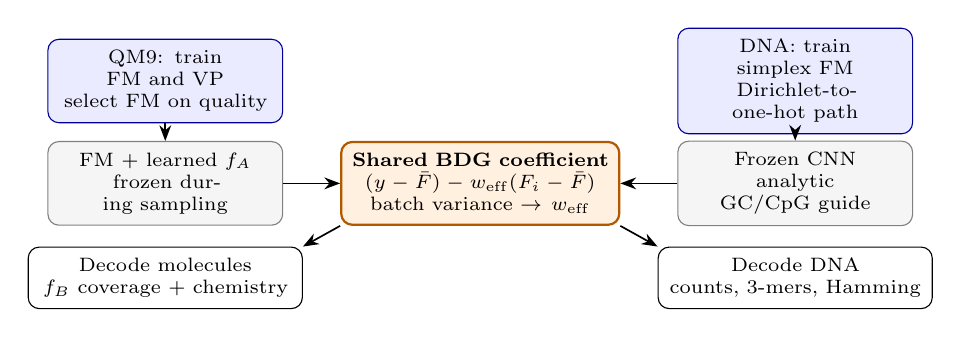
\begin{tikzpicture}[font=\scriptsize,
box/.style={draw,rounded corners,align=center,inner sep=4pt},
train/.style={box,fill=blue!8,draw=blue!60!black},
frozen/.style={box,fill=black!4,draw=black!50},
new/.style={box,fill=orange!12,draw=orange!70!black,thick},
arr/.style={-{Stealth},semithick}]
\node[train,text width=2.7cm] (fm) at (0,1.3) {QM9: train FM and VP\\select FM on quality};
\node[frozen,text width=2.7cm] (frozen) at (0,0) {FM + learned $f_A$\\frozen during sampling};
\node[new,text width=3.25cm] (bdg) at (4,0) {\textbf{Shared BDG coefficient}\\$(y-\Fbar)-\weff(F_i-\Fbar)$\\batch variance $\rightarrow\weff$};
\node[train,text width=2.7cm] (seq) at (8,1.3) {DNA: train simplex FM\\Dirichlet-to-one-hot path};
\node[frozen,text width=2.7cm] (sf) at (8,0) {Frozen CNN\\analytic GC/CpG guide};
\node[box,text width=3.2cm] (eval1) at (0,-1.2) {Decode molecules\\$f_B$ coverage + chemistry};
\node[box,text width=3.2cm] (eval2) at (8,-1.2) {Decode DNA\\counts, 3-mers, Hamming};
\draw[arr] (fm)--(frozen); \draw[arr] (seq)--(sf);
\draw[arr] (frozen)--(bdg); \draw[arr] (sf)--(bdg);
\draw[arr] (bdg.south west)--(eval1.north east); \draw[arr] (bdg.south east)--(eval2.north west);
\end{tikzpicture}
\caption{Training (blue), frozen components (gray), and shared innovation (orange). FM is carried forward from the trained-model comparison; pretrained EquiFM (flow) and EDMsecond (diffusion) provide external references.}
\label{fig:overview}
\end{figure}

\section{Results}
\subsection{Evaluation Protocol}\label{sec:protocol}
\subsubsection{Metrics}
Targets are training medians (q50). Molecular IB counts decoded samples within $\delta=2\operatorname{MAE}_{\rm cal}(f_B)$ of $y$, accompanied by stability, validity and distinct-valid yield. DNA counts exact GC/CpG with half-widths 0.008833/0.008818, plus 3-mer JSD and Hamming diversity. Coverage comparisons stay within matched tasks.
\subsubsection{Fair Comparison and Computational Budget}
Settings use three seeds, 2,000 samples each, batches of 500 and 100 Euler steps. Headline BDG uses $\eta=4$, $w=1$; ablations and DNA also use $w=4$. Molecular/sequence cells sum to 81.92/5.26 wall-clock hours including evaluation (Appendix~\ref{app:evaluation}).
\subsubsection{Statistical Reporting}
Tables show mean $\pm$ seed sd. We retain the molecular protocol's unpaired binomial approximation at $|z|\ge2.99$ (18 contrasts, two-sided family level 0.05). It ignores batch coupling and rerun noise. DNA contrasts are exploratory; the gains below also survive $z=3.16$ for 32 contrasts. Unresolved differences are not equivalence claims (Table~\ref{tab:contrasts}).

\subsection{Modality 1: Flow Matching versus Diffusion}\label{sec:fmvd}
FM's higher stability (39.7\% versus 28.8\%) and validity (75.6\% versus 66.2\%) than our VP diffusion justify carrying it forward (Table~\ref{tab:fmvd}). Pretrained EquiFM (flow matching) also exceeds EDMsecond (diffusion) on these metrics. Our models share data, architecture and training settings; selection differs (Appendix~\ref{app:training}). External checkpoints provide supporting context.
% BEGIN DATA BASE
\begin{table}[!htbp]
\centering\small
\caption{Unguided QM9, $3\times2{,}000$ samples: percentages, mean $\pm$ seed sd. Lower rows use pretrained external models. Timing includes scoring: RTX A6000 except $^*$B200 MIG; runtimes are not hardware matched.}
\label{tab:fmvd}
\begin{tabular}{lccccc}
\toprule
Generator & Mol. stable$\uparrow$ & Valid$\uparrow$ & Unique$\uparrow$ & NFE & s/sample\\
\midrule
FM, ours & $39.7\pm0.6$ & $75.6\pm1.1$ & 99.8 & 100 & 0.051\\
VP diffusion, ours & $28.8\pm1.3$ & $66.2\pm0.7$ & 99.9 & 101 & 0.048$^{*}$\\
\midrule
EquiFM (flow) & $86.2\pm0.3$ & $93.8\pm0.6$ & 99.7 & 100 & 0.086\\
EDMsecond (diffusion) & $67.2\pm1.3$ & $86.0\pm1.3$ & 99.8 & 101 & 0.087\\
\bottomrule
\end{tabular}
\end{table}
% END DATA BASE

\subsection{Modality 1: Guided versus Unguided Generation}\label{sec:guidworks}
Plug-in increased our FM's coverage from 7.83\% to 10.58\% for $\mu$ and 10.28\% to 12.63\% for gap, both above threshold (Table~\ref{tab:recent}). Stability fell by 4.08/6.15 points. The $\alpha$ gain of 1.07 points remained unresolved.

\subsection{Modality 1: Innovation Ablations}\label{sec:ablations}
We crossed four gains and four setpoints plus $\eta=0$ at two strengths/backbones. Table~\ref{tab:ablation} presents dipole $\mu$ at q50: contracting BDG lowers target error and brings the mean closer to $y$ than zero gain. Increasing $\tau_m$ broadens the distribution and adjusts band occupancy (Figure~\ref{fig:results}a). Complete numeric grids for all properties appear in Appendix~\ref{app:ablations}.
% BEGIN DATA ABLATION
\begin{table}[!htbp]
\centering\small
\caption{Numeric ablation: our FM, dipole $\mu$, q50 target $y=2.4932$ D, band $\pm0.17541$ D, $w=1$. IB is percent mean $\pm$ seed sd; MAE, mean and spread $\sigma$ are decoded, in D. Zero gain ($\eta=0$) is plug-in.}
\label{tab:ablation}
\begin{tabular}{cccccc}
\toprule
$\eta$ & $\tau_m$ & IB$\uparrow$ & MAE$\downarrow$ & Mean & $\sigma$\\
\midrule
0 & -- & $10.6\pm0.4$ & 0.969 & 2.615 & 1.209\\
4 & 0.5 & $11.2\pm1.1$ & 0.903 & 2.609 & 1.113\\
4 & 1 & $8.9\pm0.2$ & 1.133 & 2.714 & 1.434\\
8 & 0.5 & $11.9\pm0.3$ & 0.861 & 2.603 & 1.064\\
8 & 1.5 & $7.6\pm0.2$ & 1.377 & 2.858 & 1.922\\
\bottomrule
\end{tabular}
\end{table}
% END DATA ABLATION

\subsection{Modality 1: Comparison with Recent Methods}\label{sec:recent}
With $\tau_m=0.5$, BDG raises mean coverage and lowers mean absolute target error across both flow backbones and all three properties. Our FM has higher seed variability than plug-in; coverage gains remain below the protocol threshold (Table~\ref{tab:contrasts}). Comparing $\tau_m=0.5$ with $1$ shows adjustable band occupancy and stability (Table~\ref{tab:recent}). The $\eta=0$ plug-in row isolates removal of BDG's added term. TFG attains higher coverage at greater stability cost.
% BEGIN DATA M1
\begin{table}[!htbp]
\centering\small
\caption{Our FM, $w=1$: decoded IB, percent mean $\pm$ seed sd; stability in $\mu/\alpha/\mathrm{gap}$ order. Plug-in removes BDG's residual ($\eta=0$); BDG uses $\eta=4$. Recent-method rows are adaptations. Full metrics: Table~\ref{tab:full-fm}.}
\label{tab:recent}
\begin{tabular}{lcccc}
\toprule
Method & IB $\mu\uparrow$ & IB $\alpha\uparrow$ & IB gap$\uparrow$ & Mol. stable$\uparrow$\\
\midrule
Unguided & $7.8\pm0.1$ & $5.0\pm0.3$ & $10.3\pm1.0$ & 39.7 / 39.7 / 39.7\\
Plug-in ($\eta=0$) & $10.6\pm0.4$ & $6.1\pm0.3$ & $12.6\pm0.7$ & 35.6 / 37.2 / 33.6\\
TMPD-inspired & $9.0\pm0.6$ & $6.1\pm0.4$ & $11.6\pm0.9$ & 38.4 / 38.9 / 37.3\\
LGD-MC & $9.6\pm0.8$ & $5.2\pm0.4$ & $10.8\pm0.7$ & 39.9 / 39.2 / 39.5\\
TFG & $28.8\pm1.6$ & $10.5\pm0.3$ & $27.5\pm0.3$ & 24.5 / 26.8 / 14.4\\
\textbf{BDG, $\tau_m=0.5$} & $11.2\pm1.1$ & $7.0\pm0.5$ & $14.2\pm0.8$ & 35.1 / 36.4 / 30.0\\
\textbf{BDG, $\tau_m=1$} & $8.9\pm0.2$ & $5.6\pm0.5$ & $10.6\pm0.2$ & 40.5 / 37.9 / 37.6\\
\bottomrule
\end{tabular}
\end{table}
% END DATA M1

\subsection{Modality 2: Transfer of the Innovation}\label{sec:m2}
At $w=4$, BDG with $\tau_m=0.5$ increases GC/CpG coverage over plug-in by 2.32/16.83 points, with nearly unchanged Hamming diversity and higher JSD (Table~\ref{tab:m2}). At $w=1$, gains are 0.42/4.82 points; only CpG clears the exploratory threshold. Switching to $\tau_m=1$ lowers occupancy. Plug-in, TMPD and LGD-MC have identical coverage on both properties in this late window; TFG-MC differs (Appendix~\ref{app:m2}).
% BEGIN DATA M2
\begin{table}[!htbp]
\centering\small\setlength{\tabcolsep}{4pt}
\caption{DNA, $w=4$, $t\ge0.5$: decoded IB (percent mean $\pm$ seed sd); 3-mer JSD ($\times10^{-4}$) and normalized Hamming diversity in GC/CpG order. TFG-MC is a restricted adaptation. Full results: Table~\ref{tab:full-m2}.}
\label{tab:m2}
\begin{tabular}{lcccc}
\toprule
Method & GC IB$\uparrow$ & CpG IB$\uparrow$ & JSD$\downarrow$ & Hamming\\
\midrule
Unguided & $14.0\pm1.0$ & $50.2\pm1.6$ & 4.53 / 4.53 & 0.7456 / 0.7456\\
DPS-style plug-in & $14.1\pm1.0$ & $51.6\pm1.4$ & 4.61 / 4.63 & 0.7456 / 0.7456\\
TMPD-inspired & $14.1\pm1.0$ & $51.6\pm1.4$ & 4.61 / 4.63 & 0.7456 / 0.7456\\
LGD-MC & $14.1\pm1.0$ & $51.6\pm1.4$ & 4.61 / 4.63 & 0.7456 / 0.7456\\
TFG-MC adaptation & $14.1\pm1.0$ & $51.1\pm1.7$ & 4.59 / 4.58 & 0.7456 / 0.7456\\
\textbf{BDG, $\tau_m=0.5$} & $16.4\pm1.2$ & $68.5\pm1.2$ & 5.93 / 7.73 & 0.7457 / 0.7457\\
\textbf{BDG, $\tau_m=1$} & $14.1\pm1.0$ & $50.3\pm1.5$ & 4.54 / 4.52 & 0.7456 / 0.7456\\
\bottomrule
\end{tabular}
\end{table}
% END DATA M2
\begin{figure}[!t]
\centering
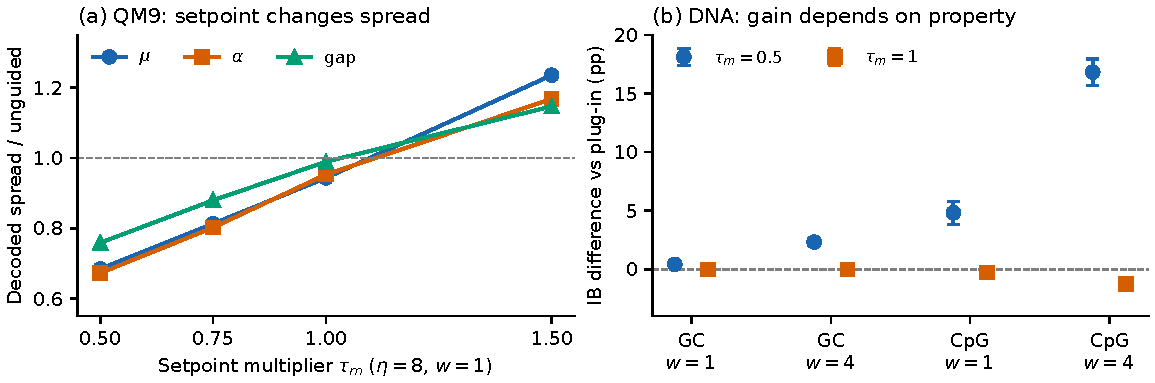
\includegraphics[width=\linewidth]{figs/results_v7.pdf}
\caption{Final-run measurements. (a) Our FM, decoded property standard deviation relative to unguided; points pool three seeds. (b) BDG minus plug-in on DNA, $\eta=4$, window $t\ge0.5$; bars show sd of three paired seed differences, not confidence intervals. Coverage scales differ by property.}
\label{fig:results}
\end{figure}

\subsection{Cross-Modality Analysis and Failure Modes}\label{sec:failure}
BDG adjusts spread and occupancy across modalities. CpG gains clear the exploratory threshold; molecular gains need more precision. Strong corrections can reduce fidelity, and GC depends on guidance timing (Appendix~\ref{app:m2}).

\section{Discussion}
Across six molecular comparisons, contracting BDG achieves higher mean coverage and lower mean absolute target error than zero-gain plug-in; the dipole ablation also brings the generated mean closer to its target. Changing $\tau_m$ adjusts decoded spread and occupancy while retaining the centering term. Positive CpG transfer extends this behavior to a second state space. These endpoint gains support BDG's added term, with measurable quality trade-offs. They do not imply faster convergence; matched-force and batch-aware analyses remain future work.
% MAIN_TEXT_END
\clearpage
\bibliographystyle{ieeetr}
\bibliography{citation,refs_extra}
\clearpage
\appendix
\renewcommand{\thetable}{S\arabic{table}}
\renewcommand{\theHtable}{S\arabic{table}}
\setcounter{table}{0}
\renewcommand{\thefigure}{S\arabic{figure}}
\renewcommand{\theHfigure}{S\arabic{figure}}
\setcounter{figure}{0}
\section{Reproducibility and Extended Results}
\subsection{Data Sources and Splits}\label{app:data}
QM9 uses the DeepChem/MoleculeNet packaging. The project retains the 3,054 entries excluded as uncharacterized in common EDM preprocessing, so published EDM dataset definitions are not identical. A seeded permutation creates the four splits stated in Section~\ref{sec:data}. Coordinates are centered, padded atoms are masked, and coordinates and one-hot features have no additional scaling. The E(3)-equivariant generator handles rotation and translation; invariant property predictors use training-derived normalization. Sizes and initial noise are shared across arms within each backend and seed. No property label enters either generator.

DeepFlyBrain is the 500-bp enhancer data used by Dirichlet FM \citep{stark2024dirichlet}. Four ambiguous training examples were excluded from the supplied 83,726. The retained splits are 83,722/10,505/10,434; channels are A/C/G/T. Class labels are unused by our unconditional generator. These random-example splits do not test sequence-cluster generalization. The older 200-bp experiment is excluded.

Exact targets and calibration values are preserved in each source cell. Molecular band half-widths for our predictor pair are 0.17541 D for $\mu$, 0.50618 Bohr$^3$ for $\alpha$, and 0.00748 Ha for gap. External EquiFM uses a different predictor pair and therefore different acceptance widths. Its coverage must not be ranked directly against our FM's coverage.

\subsection{Training and Checkpoint Records}\label{app:training}
Table~\ref{tab:training} records the training settings and evaluated checkpoints. For coordinates $c$, features $f$ and broadcast mask $M$, the training norm is
\[
\|z\|_M^2=\frac{\|M\odot z^c\|_2^2}{3\sum M}+\frac{\|M\odot z^f\|_2^2}{5\sum M}.
\]
Gaussian coordinate noise is centered; feature noise is independent Gaussian. Both molecular checkpoints specify the same split, architecture, optimizer, batch size, 1,500-epoch budget, EMA and training seed. The evaluated FM export is epoch-1500 EMA; VP is the selected epoch-1475 EMA, with validation loss 0.20784. The trainer selects validation atom stability with validation loss as a tie-breaker. The VP export records the selected epoch and configured budget, not proof of the final completed epoch. Consequently, Table~\ref{tab:fmvd} compares these trained checkpoints under shared settings with a disclosed selection difference; it does not establish family-wide superiority. VP training samples $u\in[10^{-3},1]$; its probability-flow ODE follows Equation~\eqref{eq:vp}.

\begin{table}[!htbp]
\centering\small
\caption{Training records and evaluated checkpoints. VP's selected epoch is 1475 within a configured 1500-epoch budget. Molecular predictors use one network per property and training half. Unrecorded training time is not inferred from sampling time.}
\label{tab:training}
\begin{tabular}{llll}
\toprule
Setting & Molecular FM / VP & $f_A$ / $f_B$ & Sequence FM\\
\midrule
Architecture & EGNN, 256, 8 layers & EGNN, 128, 4 & CNN, 128, 10\\
Parameters & 3.75M / 3.75M & 429,825 each & approximately 1.02M\\
Training data & \texttt{train\_a} & \texttt{train\_a}/\texttt{train\_b} & 83,722 sequences\\
Objective & velocity / noise MSE & property MSE & velocity MSE\\
Epoch budget & 1500 / 1500 & 120 & 1500 completed\\
Evaluated weights & EMA: 1500 / 1475 & validation checkpoint & epoch 1450\\
Batch size & 256 & 128 & 256\\
Optimizer & Adam & Adam & Adam\\
Initial learning rate & $2\times10^{-4}$ & $3\times10^{-4}$ & $2\times10^{-3}$\\
Schedule & cosine, floor 5\% & cosine & cosine to zero\\
EMA & 0.9999 & none & none\\
Training seed & 20260918 / 20260918 & 20260918 & 20260921\\
Training time & not fully recorded & not fully recorded & 539.7 min\\
\bottomrule
\end{tabular}
\end{table}

Sequence training performed 492,000 updates across 1,500 epochs. Validation selected update 475,600 (epoch 1450), loss 0.0633644, with 121.75M sample-views at the selected checkpoint. The total run lasted 539.7 minutes on RTX A6000, including validation. We distinguish completed training length from the selected checkpoint's age. The checkpoint uses Adam without EMA; its best-validation weights are sampled.

\begin{table}[!htbp]
\centering\small
\caption{Checkpoint fingerprints from the result records and local files. Prefixes identify artifacts; full hashes are retained in the source records.}
\label{tab:hashes}
\begin{tabular}{lll}
\toprule
Component & Identifier & Evidence\\
\midrule
Our molecular FM & MD5 \texttt{e19ccc06} & v3 cells, epoch 1500\\
Borrowed EDMsecond & MD5 \texttt{6abbd010} & v3 cells, released checkpoint\\
Sequence FM & MD5 \texttt{7f59b60b} & local checkpoint, best validation\\
Our VP diffusion & MD5 \texttt{8a3390a6} & v3 cells, epoch 1475\\
\bottomrule
\end{tabular}
\end{table}
Table~\ref{tab:hashes} identifies the evaluated artifacts. FM, EquiFM and EDMsecond cells record PyTorch 2.11.0+cu130, CUDA 13.0 and RTX A6000. VP cells record PyTorch 2.11.0+cu128, CUDA 12.8 and NVIDIA B200 MIG 2g.45gb. VP's local checkpoint MD5 matches every result cell. Hardware differs, so elapsed seconds cannot establish an FM--VP speed advantage. The sequence training report identifies RTX A6000, but individual sequence evaluation cells omit the device; those timings are not hardware-matched cross-modality benchmarks.

\subsection{Evaluation, Uncertainty, and Cost}\label{app:evaluation}
Molecular seeds are 20261001, 20261002 and 20261003. Sequence seeds are 20260921, 20260922 and 20260923. Each 2,000-sample cell contains four independent controller batches of size 500. Enlarging the total sample count adds batches, not observations to a single variance estimate. At fixed weights, seed variation measures sampling variation, not training uncertainty.

Molecular coverage counts decoded samples satisfying $|f_B(\hat x)-y|\le\delta$. Calibration uses 3,000 molecules drawn from the two training halves; each internal predictor is scored on the half it did not train on. The wrapper sets $s$ to the property standard deviation of this calibration pool, which differs from the raw predictor checkpoint's normalization scale. This $s$ sets the guidance energy and BDG setpoint; evaluator error sets $\delta$. Coverage on continuous features remains in source records but is not substituted for decoded IB.

Atom stability checks bond/valence rules; molecular stability requires every atom to pass. RDKit validity checks reconstruction and sanitization. Uniqueness divides distinct valid SMILES by valid samples; distinct-valid yield divides by all attempts. None is an energy or experimental viability measurement. IB includes invalid molecules, so usable yield requires the joint event of decoded in-band membership and stability. Marginal IB and stability cannot be multiplied to recover that event. The local aggregate results do not include the sample-level sidecars needed for this joint analysis.

The reported unpaired statistic is
\[
 z=\frac{p_a-p_b}{\sqrt{p_a(1-p_a)/6000+p_b(1-p_b)/6000}}.
\]
The registered molecular bar is 2.99. Table~\ref{tab:contrasts} reports the corresponding threshold-sized difference separately for every contrast; it is neither a power calculation nor evidence of equivalence. Within-batch dependence can invalidate an independent-Bernoulli variance, and common-noise pairing changes covariance. We retain this protocol statistic with explicit limitations and show seed standard deviations. A batch-aware paired bootstrap would need the sample-level records. At $\tau_m=0.5$, all six molecular coverage differences favor BDG in their means but remain below this bar. At $\tau_m=1$, three differences cross the bar against BDG and three remain unresolved. These outcomes distinguish an occupancy-setting effect from a universal coverage improvement. DNA uses the rule only as an exploratory comparison, and the stated positive effects survive the 32-contrast threshold of 3.16. For selections from the full molecular grid, the protocol's adjusted bar is 3.49; the paper makes descriptive grid claims without converting them into headline tests.

EquiFM same-seed reruns differ by up to 0.007 in continuous coverage. Its $\eta=0$ control agrees with plug-in only to the rerun tolerance, not bitwise. Our FM reproduces exactly. EDMsecond has same-seed variation up to 0.0015 in molecular stability. Neither binomial errors nor three seed values fully characterize this extra implementation variability.

The molecular run contains 162 headline cells, including 18 from our VP diffusion model, and 612 ablation cells. Summed recorded wall-clock is 16.77 hours for headline and 65.15 for ablations, 81.92 total. VP contributes 0.813 hours on different hardware. The DNA files contain 84 headline, 111 ablation/window and four single-seed strength cells, with 12 repeated configurations across trees; the 199 files represent 187 distinct cells and 5.26 hours of recorded compute. The repeated configurations are checked for agreement and never pooled as extra seeds. Concurrent cells and evaluation overhead prevent interpreting these totals as elapsed time or accelerator utilization.

NFE counts solver field evaluations, distinct from generator forwards and derivative calls. For each molecular flow batch, plug-in and BDG record 200 generator forwards, 50 generator VJPs, and 50 guide forward/backward pairs; unguided records 100 generator forwards. VP unguided sampling adds terminal denoising for 101 evaluations. Sequence guided batches record 150 generator forwards and 50 VJPs. BDG adds scalar reductions to plug-in, not another neural call. Equal calls do not imply equal measured runtime. Clip fractions divide clipped sample-steps by samples times guided steps \emph{per batch}; using the batch-summed step count understates them fourfold.

\subsection{Full Molecular Comparisons}\label{app:comparisons}
Tables~\ref{tab:full-fm}, \ref{tab:full-equifm}, \ref{tab:full-edm} and~\ref{tab:full-vp} report every headline arm and property. All numbers are generated by this project; no published score is mixed into these rows. EquiFM uses the released TFG guide/evaluator pair; our FM, our VP diffusion and borrowed EDMsecond use our disjoint pair. External training overlap, architectures, scales and selection differ, so all guidance contrasts stay within a backend. Equal nominal strength exposes each adaptation's behavior under shared settings; it is not a ranking of separately optimized methods.

DPS-style plug-in adapts posterior guidance to a Gaussian property energy and a flow endpoint. TMPD-inspired guidance uses a linearized uncertainty correction; LGD-MC marginalizes a local property loss; TFG combines training-free corrections. The implementations retain the local endpoint, clipping and timing choices in the cell records, and are adaptations of the cited methods, not reproductions of every original experimental setting. Molecular TFG and sequence TFG-MC are different implementations; the latter omits full TFG's iterative schedule.
% BEGIN DATA FULL-FM
\begin{table}[!htbp]
\centering\small
\caption{Complete headline evaluation on our FM. IB is decoded; IB and stability show percent mean $\pm$ seed sd. Validity and distinct-valid yield (DV) are percentages; time is recorded cell wall-clock divided by attempts. $w=1$, $t\ge0.5$, three seeds, $n=2{,}000$ each.}
\label{tab:full-fm}
\begin{tabular}{llccccc}
\toprule
Property & Method & IB$\uparrow$ & Stable$\uparrow$ & Valid$\uparrow$ & DV$\uparrow$ & s/sample\\
\midrule
$\mu$ & Unguided & $7.8\pm0.1$ & $39.7\pm0.6$ & 75.6 & 75.5 & 0.051\\
$\mu$ & DPS-style plug-in & $10.6\pm0.4$ & $35.6\pm0.3$ & 72.5 & 72.4 & 0.119\\
$\mu$ & TMPD-inspired & $9.0\pm0.6$ & $38.4\pm0.6$ & 74.8 & 74.7 & 0.255\\
$\mu$ & LGD-MC & $9.6\pm0.8$ & $39.9\pm0.3$ & 75.5 & 75.4 & 0.229\\
$\mu$ & TFG & $28.8\pm1.6$ & $24.5\pm1.0$ & 62.8 & 62.7 & 0.122\\
$\mu$ & \textbf{BDG, $\tau_m=0.5$} & $11.2\pm1.1$ & $35.1\pm1.1$ & 71.4 & 71.2 & 0.119\\
$\mu$ & \textbf{BDG, $\tau_m=1$} & $8.9\pm0.2$ & $40.5\pm0.8$ & 76.5 & 76.3 & 0.119\\
\midrule
$\alpha$ & Unguided & $5.0\pm0.3$ & $39.7\pm0.6$ & 75.6 & 75.5 & 0.050\\
$\alpha$ & DPS-style plug-in & $6.1\pm0.3$ & $37.2\pm1.6$ & 73.7 & 73.6 & 0.118\\
$\alpha$ & TMPD-inspired & $6.1\pm0.4$ & $38.9\pm1.1$ & 75.1 & 75.0 & 0.200\\
$\alpha$ & LGD-MC & $5.2\pm0.4$ & $39.2\pm1.3$ & 74.9 & 74.9 & 0.224\\
$\alpha$ & TFG & $10.5\pm0.3$ & $26.8\pm0.8$ & 61.2 & 61.1 & 0.121\\
$\alpha$ & \textbf{BDG, $\tau_m=0.5$} & $7.0\pm0.5$ & $36.4\pm1.0$ & 72.2 & 72.1 & 0.118\\
$\alpha$ & \textbf{BDG, $\tau_m=1$} & $5.6\pm0.5$ & $37.9\pm1.1$ & 75.1 & 75.1 & 0.118\\
\midrule
gap & Unguided & $10.3\pm1.0$ & $39.7\pm0.6$ & 75.6 & 75.5 & 0.051\\
gap & DPS-style plug-in & $12.6\pm0.7$ & $33.6\pm0.8$ & 69.9 & 69.8 & 0.119\\
gap & TMPD-inspired & $11.6\pm0.9$ & $37.3\pm0.7$ & 73.8 & 73.7 & 0.201\\
gap & LGD-MC & $10.8\pm0.7$ & $39.5\pm0.8$ & 75.2 & 75.1 & 0.225\\
gap & TFG & $27.5\pm0.3$ & $14.4\pm0.8$ & 45.5 & 45.5 & 0.122\\
gap & \textbf{BDG, $\tau_m=0.5$} & $14.2\pm0.8$ & $30.0\pm0.4$ & 65.8 & 65.7 & 0.119\\
gap & \textbf{BDG, $\tau_m=1$} & $10.6\pm0.2$ & $37.6\pm0.8$ & 74.3 & 74.2 & 0.119\\
\bottomrule
\end{tabular}
\end{table}
% END DATA FULL-FM
\clearpage
% BEGIN DATA FULL-EQUIFM
\begin{table}[!htbp]
\centering\small
\caption{Complete headline evaluation on borrowed EquiFM. IB is decoded; IB and stability show percent mean $\pm$ seed sd. Validity and distinct-valid yield (DV) are percentages; time is recorded cell wall-clock divided by attempts. $w=1$, $t\ge0.5$, three seeds, $n=2{,}000$ each.}
\label{tab:full-equifm}
\begin{tabular}{llccccc}
\toprule
Property & Method & IB$\uparrow$ & Stable$\uparrow$ & Valid$\uparrow$ & DV$\uparrow$ & s/sample\\
\midrule
$\mu$ & Unguided & $8.7\pm0.8$ & $86.2\pm0.3$ & 93.8 & 93.5 & 0.086\\
$\mu$ & DPS-style plug-in & $10.9\pm0.9$ & $82.1\pm0.7$ & 91.9 & 91.6 & 0.231\\
$\mu$ & TMPD-inspired & $9.0\pm0.3$ & $85.3\pm0.4$ & 93.5 & 93.2 & 0.366\\
$\mu$ & LGD-MC & $9.7\pm0.3$ & $85.5\pm0.4$ & 93.3 & 93.1 & 0.474\\
$\mu$ & TFG & $11.9\pm0.3$ & $74.0\pm0.7$ & 86.5 & 86.2 & 0.301\\
$\mu$ & \textbf{BDG, $\tau_m=0.5$} & $12.1\pm0.5$ & $79.3\pm0.7$ & 90.9 & 90.6 & 0.232\\
$\mu$ & \textbf{BDG, $\tau_m=1$} & $8.9\pm0.7$ & $85.8\pm0.3$ & 93.6 & 93.3 & 0.232\\
\midrule
$\alpha$ & Unguided & $2.1\pm0.1$ & $86.2\pm0.3$ & 93.8 & 93.5 & 0.087\\
$\alpha$ & DPS-style plug-in & $2.1\pm0.2$ & $82.9\pm0.4$ & 91.9 & 91.7 & 0.233\\
$\alpha$ & TMPD-inspired & $2.1\pm0.3$ & $84.8\pm0.3$ & 93.3 & 93.0 & 0.368\\
$\alpha$ & LGD-MC & $2.1\pm0.1$ & $85.5\pm0.9$ & 93.3 & 93.0 & 0.476\\
$\alpha$ & TFG & $3.4\pm0.5$ & $64.5\pm0.5$ & 84.5 & 84.4 & 0.302\\
$\alpha$ & \textbf{BDG, $\tau_m=0.5$} & $2.5\pm0.2$ & $76.6\pm0.5$ & 89.5 & 89.2 & 0.233\\
$\alpha$ & \textbf{BDG, $\tau_m=1$} & $2.0\pm0.1$ & $84.8\pm0.5$ & 92.8 & 92.6 & 0.233\\
\midrule
gap & Unguided & $4.9\pm0.2$ & $86.2\pm0.3$ & 93.8 & 93.5 & 0.086\\
gap & DPS-style plug-in & $5.9\pm0.3$ & $82.7\pm0.4$ & 91.9 & 91.7 & 0.231\\
gap & TMPD-inspired & $5.1\pm0.3$ & $84.6\pm0.7$ & 92.7 & 92.4 & 0.365\\
gap & LGD-MC & $5.1\pm0.4$ & $86.1\pm0.2$ & 93.5 & 93.3 & 0.473\\
gap & TFG & $10.9\pm0.2$ & $55.5\pm1.4$ & 76.4 & 76.2 & 0.300\\
gap & \textbf{BDG, $\tau_m=0.5$} & $6.8\pm0.8$ & $77.4\pm1.1$ & 90.1 & 90.0 & 0.231\\
gap & \textbf{BDG, $\tau_m=1$} & $5.0\pm0.4$ & $85.6\pm0.3$ & 93.4 & 93.1 & 0.231\\
\bottomrule
\end{tabular}
\end{table}
% END DATA FULL-EQUIFM
% BEGIN DATA FULL-EDM
\begin{table}[!htbp]
\centering\small
\caption{Complete headline evaluation on borrowed EDMsecond. IB is decoded; IB and stability show percent mean $\pm$ seed sd. Validity and distinct-valid yield (DV) are percentages; time is recorded cell wall-clock divided by attempts. $w=1$, $t\ge0.5$, three seeds, $n=2{,}000$ each.}
\label{tab:full-edm}
\begin{tabular}{llccccc}
\toprule
Property & Method & IB$\uparrow$ & Stable$\uparrow$ & Valid$\uparrow$ & DV$\uparrow$ & s/sample\\
\midrule
$\mu$ & Unguided & $9.4\pm0.2$ & $67.2\pm1.3$ & 86.0 & 85.8 & 0.087\\
$\mu$ & DPS-style plug-in & $11.2\pm1.1$ & $62.2\pm0.6$ & 82.8 & 82.7 & 0.210\\
\midrule
$\alpha$ & Unguided & $5.4\pm0.7$ & $67.2\pm1.2$ & 86.0 & 85.8 & 0.087\\
$\alpha$ & DPS-style plug-in & $6.1\pm0.4$ & $64.6\pm0.8$ & 84.1 & 83.9 & 0.208\\
\midrule
gap & Unguided & $10.8\pm0.7$ & $67.1\pm1.3$ & 86.0 & 85.8 & 0.087\\
gap & DPS-style plug-in & $12.8\pm0.7$ & $57.9\pm1.7$ & 80.3 & 80.2 & 0.209\\
\bottomrule
\end{tabular}
\end{table}
% END DATA FULL-EDM
\clearpage
% BEGIN DATA FULL-VP
\begin{table}[!htbp]
\centering\small
\caption{Complete headline evaluation on our VP diffusion. IB is decoded; IB and stability show percent mean $\pm$ seed sd. Validity and distinct-valid yield (DV) are percentages; time is recorded cell wall-clock divided by attempts. $w=1$, $t\ge0.5$, three seeds, $n=2{,}000$ each.}
\label{tab:full-vp}
\begin{tabular}{llccccc}
\toprule
Property & Method & IB$\uparrow$ & Stable$\uparrow$ & Valid$\uparrow$ & DV$\uparrow$ & s/sample\\
\midrule
$\mu$ & Unguided & $8.7\pm0.8$ & $28.8\pm1.3$ & 66.2 & 66.1 & 0.048\\
$\mu$ & DPS-style plug-in & $10.8\pm0.4$ & $26.2\pm0.9$ & 61.8 & 61.7 & 0.114\\
\midrule
$\alpha$ & Unguided & $5.2\pm0.6$ & $28.8\pm1.3$ & 66.2 & 66.1 & 0.048\\
$\alpha$ & DPS-style plug-in & $5.4\pm0.4$ & $25.2\pm1.5$ & 58.7 & 58.6 & 0.114\\
\midrule
gap & Unguided & $9.8\pm0.6$ & $28.8\pm1.3$ & 66.2 & 66.1 & 0.048\\
gap & DPS-style plug-in & $12.4\pm1.2$ & $23.2\pm0.6$ & 57.3 & 57.3 & 0.114\\
\bottomrule
\end{tabular}
\end{table}
% END DATA FULL-VP
% BEGIN DATA CONTRASTS
\begin{table}[!htbp]
\centering\small
\caption{BDG minus plug-in on decoded molecular IB. Differences, paired seed sd and the threshold-sized difference $2.99\,\mathrm{se}(\Delta)$ are in percentage points. The registered unpaired statistic is shown separately from descriptive pairing.}
\label{tab:contrasts}
\begin{tabular}{llccccc}
\toprule
Backend & Property & $\tau_m$ & $\Delta$IB & SD$(\Delta)$ & $z$ & Threshold\\
\midrule
fm & $\mu$ & 0.5 & +0.63 & 1.45 & +1.11 & 1.70\\
fm & $\mu$ & 1 & -1.68 & 0.19 & -3.11 & 1.62\\
fm & $\alpha$ & 0.5 & +0.90 & 0.50 & +2.00 & 1.35\\
fm & $\alpha$ & 1 & -0.43 & 0.75 & -1.01 & 1.28\\
fm & gap & 0.5 & +1.52 & 0.21 & +2.44 & 1.86\\
fm & gap & 1 & -2.07 & 0.72 & -3.54 & 1.75\\
equifm & $\mu$ & 0.5 & +1.25 & 0.70 & +2.15 & 1.74\\
equifm & $\mu$ & 1 & -1.93 & 0.62 & -3.55 & 1.63\\
equifm & $\alpha$ & 0.5 & +0.45 & 0.13 & +1.65 & 0.81\\
equifm & $\alpha$ & 1 & -0.02 & 0.31 & -0.06 & 0.77\\
equifm & gap & 0.5 & +0.90 & 0.56 & +2.02 & 1.33\\
equifm & gap & 1 & -0.93 & 0.67 & -2.25 & 1.24\\
\bottomrule
\end{tabular}
\end{table}
% END DATA CONTRASTS

\subsection{Complete Molecular Ablation Grids}\label{app:ablations}
Figures~\ref{fig:abl-fm} and~\ref{fig:abl-equifm} show every nonzero gain/setpoint combination as decoded coverage change from its own zero-gain control, with strengths kept separate. Tables~\ref{tab:grid-fm-mu}, \ref{tab:grid-fm-alpha}, \ref{tab:grid-fm-gap}, \ref{tab:grid-equifm-mu}, \ref{tab:grid-equifm-alpha} and~\ref{tab:grid-equifm-gap} provide the complete numeric ablations: 204 configurations, each evaluated with three seeds, accounting for all 612 cells. Each caption specifies its property, q50 target and band. These tables extend the selected dipole rows in Table~\ref{tab:ablation} with both strengths, all gains and setpoints, target error, bias, spread and stability.

For our FM dipole task at $w=1$, zero gain gives MAE 0.969 D and pooled mean 2.615 D around $y=2.4932$ D. At $\tau_m=0.5$, gains 4 and 8 lower MAE to 0.903 and 0.861 D and move the mean to 2.609 and 2.603 D. This supports improved endpoint target concentration in the selected ablation. Mean bias is not uniformly improved across properties: our FM gap bias grows slightly in magnitude at gain 4 despite lower MAE. Increasing gain also need not monotonically increase coverage, especially at $w=4$. The wider setpoint lowers occupancy of the fixed band in every grid, illustrating the intended spread--occupancy trade-off.

At $\eta=8,w=1,\tau_m=1.5$, decoded spread exceeds unguided for all three properties and both flow backends, approximately 1.15--1.25 times the reference. The tested positive plug-in strengths $w\in\{1,4\}$ remain below it. This comparison does not exclude signed strengths, arbitrary schedules, or a shifted plug-in target from reaching similar states. One-sided residuals, open-loop replay and signed-strength controls were not part of the completed grid.
\begin{figure}[!htbp]
\centering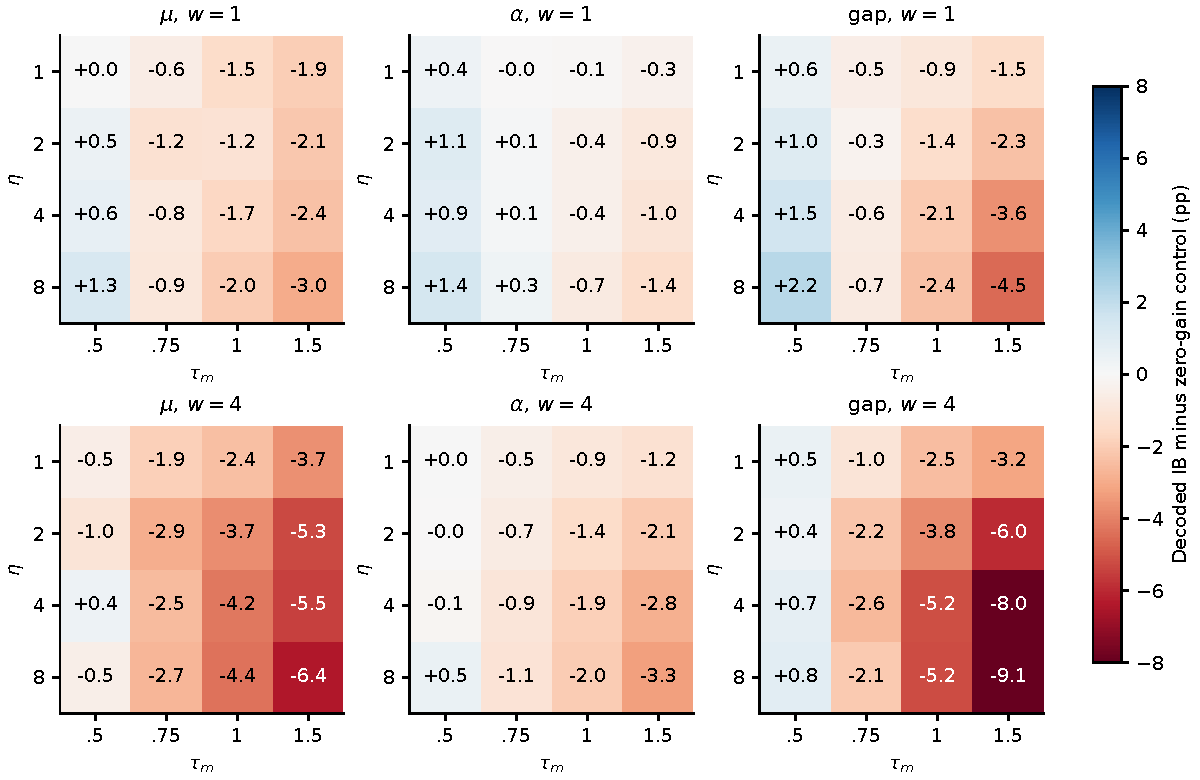
\includegraphics[width=\linewidth]{figs/ablation_fm_v7.pdf}
\caption{Our FM: full decoded coverage ablation. Each panel fixes property and strength; entries are percentage-point changes from $\eta=0$ at that strength. The color scale is shared with Figure~\ref{fig:abl-equifm}; values outside its range retain their exact text.}
\label{fig:abl-fm}
\end{figure}
\begin{figure}[!htbp]
\centering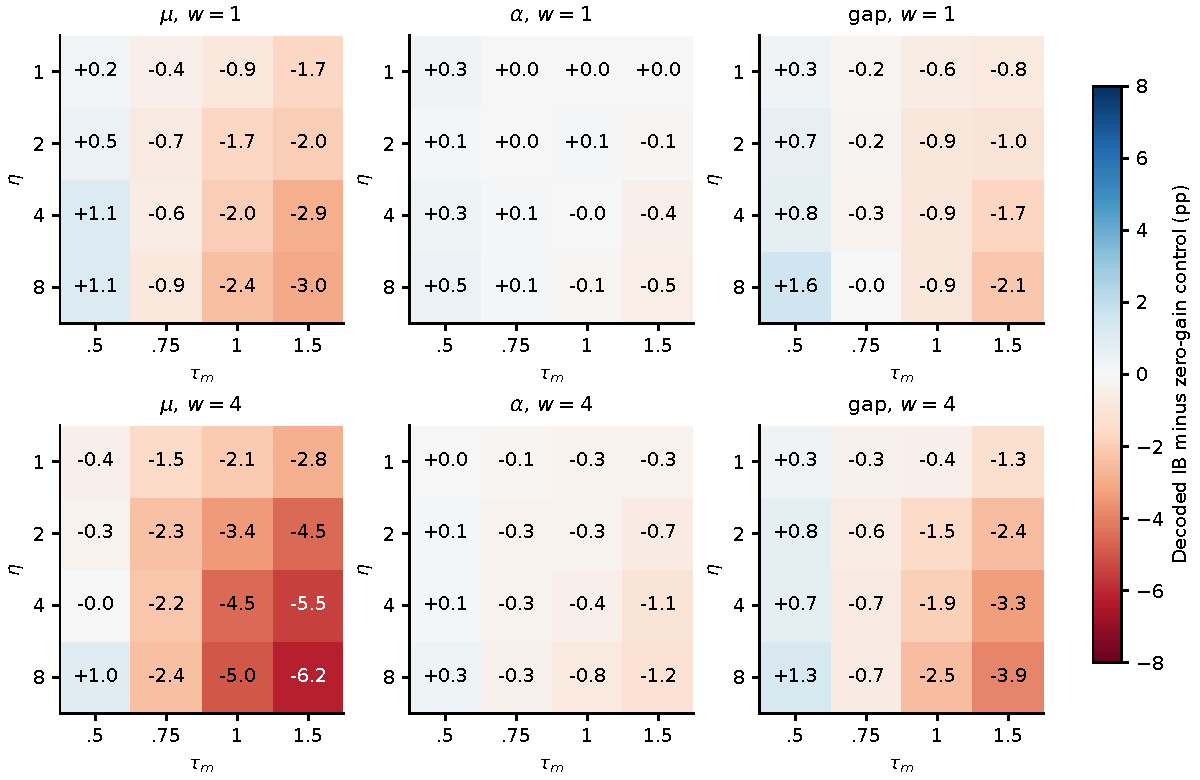
\includegraphics[width=\linewidth]{figs/ablation_equifm_v7.pdf}
\caption{Borrowed EquiFM: the same complete grid and matched zero-gain contrasts. Rerun variability accompanies the three-seed averages.}
\label{fig:abl-equifm}
\end{figure}
\clearpage
% BEGIN DATA GRID-FM-MU
\begin{table}[!htbp]
\centering\small
\caption{Our FM, $\mu$: all gain/setpoint ablations at $w=1,4$, q50 target $y=2.4932$ D, half-width $\delta=0.17541$ D. Each row uses three seeds of 2,000 samples. IB and molecular stability are percent mean $\pm$ seed sd. MAE, signed bias of the pooled mean, and pooled standard deviation $\sigma$ are decoded and normalized by $\delta$. The $\eta=0$ row removes the residual; its setpoint is irrelevant.}
\label{tab:grid-fm-mu}
\begin{tabular}{cccccccc}
\toprule
$w$ & $\eta$ & $\tau_m$ & IB$\uparrow$ & MAE/$\delta\downarrow$ & Bias/$\delta$ & $\sigma/\delta$ & Stable$\uparrow$\\
\midrule
1 & 0 & -- & $10.6\pm0.4$ & 5.53 & +0.69 & 6.89 & $35.6\pm0.3$\\
1 & 1 & 0.5 & $10.6\pm0.2$ & 5.42 & +0.75 & 6.74 & $35.7\pm0.2$\\
1 & 1 & 0.75 & $10.0\pm0.0$ & 5.77 & +0.89 & 7.13 & $37.8\pm0.5$\\
1 & 1 & 1 & $9.1\pm0.1$ & 6.00 & +1.03 & 7.45 & $38.9\pm1.2$\\
1 & 1 & 1.5 & $8.6\pm0.2$ & 6.24 & +1.21 & 7.81 & $39.2\pm0.7$\\
1 & 2 & 0.5 & $11.1\pm0.5$ & 5.30 & +0.70 & 6.56 & $35.8\pm0.5$\\
1 & 2 & 0.75 & $9.4\pm0.3$ & 5.90 & +1.01 & 7.33 & $38.8\pm1.2$\\
1 & 2 & 1 & $9.4\pm0.4$ & 6.23 & +1.25 & 7.77 & $39.6\pm0.4$\\
1 & 2 & 1.5 & $8.5\pm0.5$ & 6.81 & +1.45 & 8.82 & $39.4\pm0.9$\\
1 & 4 & 0.5 & $11.2\pm1.1$ & 5.15 & +0.66 & 6.35 & $35.1\pm1.1$\\
1 & 4 & 0.75 & $9.8\pm0.5$ & 5.91 & +1.03 & 7.30 & $38.9\pm0.3$\\
1 & 4 & 1 & $8.9\pm0.2$ & 6.46 & +1.26 & 8.17 & $40.5\pm0.8$\\
1 & 4 & 1.5 & $8.2\pm0.7$ & 7.27 & +1.71 & 9.93 & $38.2\pm1.0$\\
1 & 8 & 0.5 & $11.9\pm0.3$ & 4.91 & +0.62 & 6.07 & $34.0\pm0.5$\\
1 & 8 & 0.75 & $9.7\pm0.4$ & 5.82 & +1.02 & 7.21 & $38.7\pm0.5$\\
1 & 8 & 1 & $8.6\pm0.4$ & 6.64 & +1.37 & 8.36 & $40.4\pm0.7$\\
1 & 8 & 1.5 & $7.6\pm0.2$ & 7.85 & +2.08 & 10.96 & $37.6\pm1.2$\\
\midrule
4 & 0 & -- & $13.4\pm0.4$ & 4.63 & +0.31 & 5.84 & $30.3\pm0.6$\\
4 & 1 & 0.5 & $12.9\pm0.5$ & 4.70 & +0.27 & 5.85 & $31.2\pm0.5$\\
4 & 1 & 0.75 & $11.6\pm0.5$ & 5.10 & +0.44 & 6.31 & $34.3\pm0.4$\\
4 & 1 & 1 & $11.0\pm0.3$ & 5.33 & +0.58 & 6.60 & $35.4\pm0.7$\\
4 & 1 & 1.5 & $9.8\pm0.2$ & 5.76 & +0.72 & 7.15 & $38.1\pm1.4$\\
4 & 2 & 0.5 & $12.4\pm0.8$ & 4.64 & +0.28 & 5.72 & $31.8\pm0.3$\\
4 & 2 & 0.75 & $10.5\pm0.7$ & 5.40 & +0.62 & 6.71 & $36.0\pm1.1$\\
4 & 2 & 1 & $9.7\pm0.4$ & 5.88 & +0.75 & 7.30 & $39.1\pm0.9$\\
4 & 2 & 1.5 & $8.1\pm0.8$ & 6.76 & +1.09 & 8.79 & $38.6\pm1.2$\\
4 & 4 & 0.5 & $13.8\pm0.4$ & 4.50 & +0.34 & 5.58 & $33.5\pm0.6$\\
4 & 4 & 0.75 & $10.9\pm0.6$ & 5.40 & +0.58 & 6.70 & $37.4\pm1.0$\\
4 & 4 & 1 & $9.2\pm0.6$ & 6.28 & +0.82 & 7.83 & $39.9\pm0.2$\\
4 & 4 & 1.5 & $8.0\pm0.3$ & 7.61 & +1.40 & 10.44 & $36.6\pm1.0$\\
4 & 8 & 0.5 & $13.0\pm0.5$ & 4.46 & +0.49 & 5.54 & $34.0\pm1.6$\\
4 & 8 & 0.75 & $10.8\pm0.3$ & 5.42 & +1.01 & 6.81 & $37.7\pm0.5$\\
4 & 8 & 1 & $9.1\pm0.8$ & 6.41 & +1.01 & 8.09 & $40.3\pm0.7$\\
4 & 8 & 1.5 & $7.0\pm0.2$ & 8.05 & +1.55 & 11.08 & $37.5\pm0.6$\\
\bottomrule
\end{tabular}
\end{table}
% END DATA GRID-FM-MU
\clearpage
% BEGIN DATA GRID-FM-ALPHA
\begin{table}[!htbp]
\centering\small
\caption{Our FM, $\alpha$: all gain/setpoint ablations at $w=1,4$, q50 target $y=75.5400$ Bohr$^3$, half-width $\delta=0.50618$ Bohr$^3$. Each row uses three seeds of 2,000 samples. IB and molecular stability are percent mean $\pm$ seed sd. MAE, signed bias of the pooled mean, and pooled standard deviation $\sigma$ are decoded and normalized by $\delta$. The $\eta=0$ row removes the residual; its setpoint is irrelevant.}
\label{tab:grid-fm-alpha}
\begin{tabular}{cccccccc}
\toprule
$w$ & $\eta$ & $\tau_m$ & IB$\uparrow$ & MAE/$\delta\downarrow$ & Bias/$\delta$ & $\sigma/\delta$ & Stable$\uparrow$\\
\midrule
1 & 0 & -- & $6.1\pm0.3$ & 10.47 & +1.79 & 13.23 & $37.2\pm1.6$\\
1 & 1 & 0.5 & $6.5\pm0.1$ & 9.65 & +1.74 & 12.30 & $37.7\pm1.8$\\
1 & 1 & 0.75 & $6.1\pm0.2$ & 10.53 & +1.81 & 13.30 & $37.8\pm1.6$\\
1 & 1 & 1 & $6.0\pm0.0$ & 11.12 & +1.69 & 14.05 & $37.8\pm1.3$\\
1 & 1 & 1.5 & $5.8\pm0.4$ & 11.74 & +1.64 & 14.91 & $38.3\pm1.0$\\
1 & 2 & 0.5 & $7.1\pm0.6$ & 9.29 & +1.77 & 11.90 & $37.0\pm1.1$\\
1 & 2 & 0.75 & $6.2\pm0.4$ & 10.56 & +1.82 & 13.34 & $37.8\pm1.3$\\
1 & 2 & 1 & $5.7\pm0.3$ & 11.59 & +1.71 & 14.67 & $38.5\pm0.5$\\
1 & 2 & 1.5 & $5.2\pm0.2$ & 12.72 & +1.16 & 16.39 & $38.3\pm0.7$\\
1 & 4 & 0.5 & $7.0\pm0.5$ & 9.00 & +1.78 & 11.56 & $36.4\pm1.0$\\
1 & 4 & 0.75 & $6.2\pm0.2$ & 10.56 & +1.80 & 13.34 & $37.6\pm1.2$\\
1 & 4 & 1 & $5.6\pm0.5$ & 11.99 & +1.58 & 15.24 & $37.9\pm1.1$\\
1 & 4 & 1.5 & $5.1\pm0.4$ & 13.61 & +0.57 & 17.81 & $37.8\pm0.4$\\
1 & 8 & 0.5 & $7.5\pm0.4$ & 8.67 & +1.75 & 11.16 & $35.5\pm0.3$\\
1 & 8 & 0.75 & $6.4\pm0.1$ & 10.52 & +1.81 & 13.31 & $37.9\pm1.7$\\
1 & 8 & 1 & $5.4\pm0.3$ & 12.39 & +1.40 & 15.81 & $38.2\pm0.5$\\
1 & 8 & 1.5 & $4.7\pm0.4$ & 14.69 & +0.04 & 19.38 & $37.3\pm0.3$\\
\midrule
4 & 0 & -- & $7.5\pm0.4$ & 8.58 & +2.85 & 10.81 & $34.1\pm1.1$\\
4 & 1 & 0.5 & $7.5\pm0.2$ & 8.53 & +2.93 & 10.71 & $33.2\pm1.0$\\
4 & 1 & 0.75 & $7.0\pm0.1$ & 9.32 & +2.99 & 11.66 & $35.9\pm0.1$\\
4 & 1 & 1 & $6.6\pm0.4$ & 9.89 & +3.06 & 12.31 & $36.4\pm1.1$\\
4 & 1 & 1.5 & $6.3\pm0.4$ & 10.71 & +2.94 & 13.35 & $37.6\pm0.8$\\
4 & 2 & 0.5 & $7.4\pm0.1$ & 8.49 & +2.97 & 10.61 & $33.4\pm1.0$\\
4 & 2 & 0.75 & $6.8\pm0.2$ & 9.75 & +3.12 & 12.12 & $36.5\pm0.4$\\
4 & 2 & 1 & $6.0\pm0.5$ & 10.97 & +2.99 & 13.66 & $37.9\pm0.7$\\
4 & 2 & 1.5 & $5.4\pm0.4$ & 12.74 & +2.22 & 16.31 & $38.2\pm0.4$\\
4 & 4 & 0.5 & $7.3\pm0.1$ & 8.38 & +2.94 & 10.42 & $33.5\pm0.9$\\
4 & 4 & 0.75 & $6.5\pm0.4$ & 10.10 & +3.09 & 12.52 & $36.8\pm0.8$\\
4 & 4 & 1 & $5.6\pm0.3$ & 11.80 & +2.77 & 14.86 & $38.1\pm1.0$\\
4 & 4 & 1.5 & $4.6\pm0.3$ & 14.33 & +1.20 & 18.70 & $36.8\pm1.3$\\
4 & 8 & 0.5 & $8.0\pm0.5$ & 8.21 & +2.93 & 10.23 & $33.1\pm0.1$\\
4 & 8 & 0.75 & $6.4\pm0.4$ & 10.27 & +3.08 & 12.73 & $37.2\pm0.9$\\
4 & 8 & 1 & $5.4\pm0.1$ & 12.26 & +2.51 & 15.68 & $38.8\pm0.9$\\
4 & 8 & 1.5 & $4.2\pm0.3$ & 16.11 & +0.49 & 20.85 & $35.8\pm0.8$\\
\bottomrule
\end{tabular}
\end{table}
% END DATA GRID-FM-ALPHA
\clearpage
% BEGIN DATA GRID-FM-GAP
\begin{table}[!htbp]
\centering\small
\caption{Our FM, gap: all gain/setpoint ablations at $w=1,4$, q50 target $y=0.2496$ Ha, half-width $\delta=0.00748$ Ha. Each row uses three seeds of 2,000 samples. IB and molecular stability are percent mean $\pm$ seed sd. MAE, signed bias of the pooled mean, and pooled standard deviation $\sigma$ are decoded and normalized by $\delta$. The $\eta=0$ row removes the residual; its setpoint is irrelevant.}
\label{tab:grid-fm-gap}
\begin{tabular}{cccccccc}
\toprule
$w$ & $\eta$ & $\tau_m$ & IB$\uparrow$ & MAE/$\delta\downarrow$ & Bias/$\delta$ & $\sigma/\delta$ & Stable$\uparrow$\\
\midrule
1 & 0 & -- & $12.6\pm0.7$ & 4.51 & -1.26 & 5.29 & $33.6\pm0.8$\\
1 & 1 & 0.5 & $13.2\pm0.7$ & 4.36 & -1.30 & 5.12 & $31.3\pm0.6$\\
1 & 1 & 0.75 & $12.1\pm0.8$ & 4.57 & -1.25 & 5.37 & $34.1\pm0.3$\\
1 & 1 & 1 & $11.8\pm1.1$ & 4.74 & -1.26 & 5.56 & $36.6\pm0.6$\\
1 & 1 & 1.5 & $11.2\pm0.7$ & 4.95 & -1.18 & 5.81 & $37.6\pm0.1$\\
1 & 2 & 0.5 & $13.7\pm0.5$ & 4.24 & -1.37 & 4.95 & $31.0\pm0.9$\\
1 & 2 & 0.75 & $12.4\pm0.9$ & 4.60 & -1.29 & 5.40 & $35.0\pm1.3$\\
1 & 2 & 1 & $11.3\pm0.8$ & 4.90 & -1.21 & 5.75 & $37.4\pm0.9$\\
1 & 2 & 1.5 & $10.3\pm0.4$ & 5.31 & -1.15 & 6.24 & $38.2\pm0.7$\\
1 & 4 & 0.5 & $14.2\pm0.8$ & 4.13 & -1.36 & 4.82 & $30.0\pm0.4$\\
1 & 4 & 0.75 & $12.0\pm0.4$ & 4.62 & -1.31 & 5.40 & $35.1\pm1.0$\\
1 & 4 & 1 & $10.6\pm0.2$ & 5.09 & -1.17 & 5.95 & $37.6\pm0.8$\\
1 & 4 & 1.5 & $9.0\pm0.5$ & 5.70 & -1.01 & 6.69 & $35.3\pm0.4$\\
1 & 8 & 0.5 & $14.8\pm0.8$ & 3.96 & -1.28 & 4.64 & $29.3\pm0.5$\\
1 & 8 & 0.75 & $11.9\pm0.2$ & 4.58 & -1.19 & 5.38 & $35.4\pm0.7$\\
1 & 8 & 1 & $10.3\pm0.4$ & 5.16 & -1.19 & 6.05 & $37.4\pm0.6$\\
1 & 8 & 1.5 & $8.1\pm0.5$ & 6.01 & -0.87 & 7.02 & $33.0\pm1.5$\\
\midrule
4 & 0 & -- & $15.6\pm0.8$ & 3.89 & -1.14 & 4.63 & $25.8\pm0.8$\\
4 & 1 & 0.5 & $16.1\pm0.7$ & 3.84 & -1.23 & 4.55 & $25.4\pm0.4$\\
4 & 1 & 0.75 & $14.6\pm0.5$ & 4.11 & -1.24 & 4.85 & $28.8\pm1.1$\\
4 & 1 & 1 & $13.1\pm0.4$ & 4.36 & -1.23 & 5.13 & $30.8\pm1.0$\\
4 & 1 & 1.5 & $12.5\pm0.1$ & 4.60 & -1.26 & 5.39 & $33.7\pm1.0$\\
4 & 2 & 0.5 & $16.0\pm0.4$ & 3.80 & -1.23 & 4.49 & $25.4\pm0.7$\\
4 & 2 & 0.75 & $13.4\pm0.7$ & 4.28 & -1.25 & 5.05 & $30.2\pm0.7$\\
4 & 2 & 1 & $11.9\pm0.2$ & 4.65 & -1.19 & 5.47 & $34.9\pm0.6$\\
4 & 2 & 1.5 & $9.6\pm0.3$ & 5.40 & -1.10 & 6.34 & $36.5\pm0.7$\\
4 & 4 & 0.5 & $16.4\pm0.4$ & 3.74 & -1.20 & 4.42 & $27.0\pm0.3$\\
4 & 4 & 0.75 & $13.0\pm0.4$ & 4.35 & -1.14 & 5.14 & $33.0\pm1.4$\\
4 & 4 & 1 & $10.5\pm0.8$ & 4.96 & -1.08 & 5.83 & $36.6\pm0.6$\\
4 & 4 & 1.5 & $7.6\pm0.6$ & 6.06 & -0.90 & 7.05 & $33.7\pm1.1$\\
4 & 8 & 0.5 & $16.5\pm0.4$ & 3.67 & -0.97 & 4.41 & $27.0\pm0.6$\\
4 & 8 & 0.75 & $13.5\pm1.1$ & 4.39 & -0.96 & 5.24 & $34.1\pm0.3$\\
4 & 8 & 1 & $10.4\pm0.2$ & 5.08 & -1.05 & 5.97 & $38.1\pm0.6$\\
4 & 8 & 1.5 & $6.5\pm0.6$ & 6.47 & -0.77 & 7.47 & $31.5\pm1.6$\\
\bottomrule
\end{tabular}
\end{table}
% END DATA GRID-FM-GAP
\clearpage
% BEGIN DATA GRID-EQUIFM-MU
\begin{table}[!htbp]
\centering\small
\caption{Pretrained EquiFM (flow matching), $\mu$: all gain/setpoint ablations at $w=1,4$, q50 target $y=2.4932$ D, half-width $\delta=0.15675$ D. Each row uses three seeds of 2,000 samples. IB and molecular stability are percent mean $\pm$ seed sd. MAE, signed bias of the pooled mean, and pooled standard deviation $\sigma$ are decoded and normalized by $\delta$. The $\eta=0$ row removes the residual; its setpoint is irrelevant.}
\label{tab:grid-equifm-mu}
\begin{tabular}{cccccccc}
\toprule
$w$ & $\eta$ & $\tau_m$ & IB$\uparrow$ & MAE/$\delta\downarrow$ & Bias/$\delta$ & $\sigma/\delta$ & Stable$\uparrow$\\
\midrule
1 & 0 & -- & $10.9\pm0.9$ & 5.71 & +1.27 & 7.17 & $81.9\pm0.9$\\
1 & 1 & 0.5 & $11.1\pm0.9$ & 5.45 & +1.03 & 6.79 & $80.9\pm0.5$\\
1 & 1 & 0.75 & $10.5\pm1.0$ & 5.84 & +1.28 & 7.28 & $82.6\pm1.1$\\
1 & 1 & 1 & $10.1\pm1.0$ & 6.09 & +1.46 & 7.59 & $83.6\pm1.2$\\
1 & 1 & 1.5 & $9.2\pm0.9$ & 6.41 & +1.74 & 7.99 & $85.0\pm0.9$\\
1 & 2 & 0.5 & $11.4\pm0.5$ & 5.38 & +1.02 & 6.73 & $80.0\pm0.9$\\
1 & 2 & 0.75 & $10.2\pm0.7$ & 5.97 & +1.40 & 7.48 & $83.5\pm1.2$\\
1 & 2 & 1 & $9.2\pm0.2$ & 6.42 & +1.72 & 7.97 & $84.9\pm0.5$\\
1 & 2 & 1.5 & $9.0\pm0.4$ & 7.11 & +2.03 & 9.68 & $85.4\pm0.6$\\
1 & 4 & 0.5 & $12.0\pm0.3$ & 5.22 & +0.85 & 6.58 & $79.0\pm0.2$\\
1 & 4 & 0.75 & $10.3\pm0.1$ & 6.00 & +1.39 & 7.50 & $84.1\pm1.0$\\
1 & 4 & 1 & $8.9\pm0.7$ & 6.70 & +1.83 & 8.52 & $85.5\pm0.3$\\
1 & 4 & 1.5 & $8.0\pm0.1$ & 7.60 & +2.21 & 10.50 & $83.0\pm0.9$\\
1 & 8 & 0.5 & $12.0\pm0.2$ & 5.08 & +0.84 & 6.31 & $79.0\pm0.9$\\
1 & 8 & 0.75 & $10.1\pm0.6$ & 6.01 & +1.36 & 7.43 & $84.7\pm0.5$\\
1 & 8 & 1 & $8.5\pm0.7$ & 6.96 & +2.00 & 8.87 & $85.4\pm0.6$\\
1 & 8 & 1.5 & $7.9\pm0.3$ & 8.02 & +2.41 & 11.38 & $82.0\pm0.7$\\
\midrule
4 & 0 & -- & $13.2\pm0.5$ & 4.77 & +0.59 & 6.07 & $75.6\pm0.6$\\
4 & 1 & 0.5 & $12.8\pm0.7$ & 4.79 & +0.68 & 6.00 & $75.9\pm0.7$\\
4 & 1 & 0.75 & $11.7\pm0.7$ & 5.21 & +0.86 & 6.54 & $78.7\pm0.8$\\
4 & 1 & 1 & $11.1\pm1.2$ & 5.46 & +0.96 & 6.82 & $80.9\pm0.7$\\
4 & 1 & 1.5 & $10.4\pm0.9$ & 5.77 & +1.08 & 7.24 & $83.1\pm0.7$\\
4 & 2 & 0.5 & $12.9\pm1.0$ & 4.78 & +0.64 & 6.01 & $76.1\pm1.3$\\
4 & 2 & 0.75 & $10.9\pm0.6$ & 5.46 & +0.98 & 6.82 & $81.3\pm0.3$\\
4 & 2 & 1 & $9.8\pm0.4$ & 6.00 & +1.21 & 7.41 & $84.8\pm0.6$\\
4 & 2 & 1.5 & $8.7\pm0.9$ & 7.06 & +1.59 & 9.34 & $84.8\pm1.0$\\
4 & 4 & 0.5 & $13.2\pm0.7$ & 4.70 & +0.55 & 5.88 & $76.5\pm0.4$\\
4 & 4 & 0.75 & $11.0\pm0.7$ & 5.62 & +1.07 & 7.03 & $83.3\pm0.7$\\
4 & 4 & 1 & $8.7\pm0.5$ & 6.52 & +1.33 & 8.16 & $85.5\pm0.8$\\
4 & 4 & 1.5 & $7.8\pm0.2$ & 7.84 & +1.81 & 10.95 & $81.7\pm0.7$\\
4 & 8 & 0.5 & $14.2\pm0.2$ & 4.60 & +0.49 & 5.87 & $78.5\pm0.4$\\
4 & 8 & 0.75 & $10.8\pm0.4$ & 5.69 & +1.13 & 7.17 & $83.4\pm0.7$\\
4 & 8 & 1 & $8.2\pm0.5$ & 6.87 & +1.58 & 8.72 & $85.2\pm0.8$\\
4 & 8 & 1.5 & $7.0\pm0.3$ & 8.25 & +1.93 & 11.54 & $81.2\pm0.6$\\
\bottomrule
\end{tabular}
\end{table}
% END DATA GRID-EQUIFM-MU
\clearpage
% BEGIN DATA GRID-EQUIFM-ALPHA
\begin{table}[!htbp]
\centering\small
\caption{Pretrained EquiFM (flow matching), $\alpha$: all gain/setpoint ablations at $w=1,4$, q50 target $y=75.5400$ Bohr$^3$, half-width $\delta=0.16480$ Bohr$^3$. Each row uses three seeds of 2,000 samples. IB and molecular stability are percent mean $\pm$ seed sd. MAE, signed bias of the pooled mean, and pooled standard deviation $\sigma$ are decoded and normalized by $\delta$. The $\eta=0$ row removes the residual; its setpoint is irrelevant.}
\label{tab:grid-equifm-alpha}
\begin{tabular}{cccccccc}
\toprule
$w$ & $\eta$ & $\tau_m$ & IB$\uparrow$ & MAE/$\delta\downarrow$ & Bias/$\delta$ & $\sigma/\delta$ & Stable$\uparrow$\\
\midrule
1 & 0 & -- & $2.1\pm0.2$ & 32.49 & -11.31 & 41.35 & $82.8\pm0.4$\\
1 & 1 & 0.5 & $2.3\pm0.3$ & 30.38 & -11.58 & 38.68 & $80.5\pm1.0$\\
1 & 1 & 0.75 & $2.1\pm0.2$ & 32.16 & -11.25 & 40.89 & $82.7\pm0.6$\\
1 & 1 & 1 & $2.1\pm0.1$ & 33.29 & -10.91 & 42.32 & $83.9\pm1.0$\\
1 & 1 & 1.5 & $2.1\pm0.2$ & 34.74 & -11.02 & 44.12 & $85.0\pm0.6$\\
1 & 2 & 0.5 & $2.2\pm0.4$ & 29.62 & -11.95 & 37.43 & $78.9\pm1.1$\\
1 & 2 & 0.75 & $2.1\pm0.3$ & 31.97 & -11.30 & 40.62 & $82.7\pm0.1$\\
1 & 2 & 1 & $2.1\pm0.1$ & 34.28 & -10.96 & 43.51 & $84.7\pm0.5$\\
1 & 2 & 1.5 & $2.0\pm0.3$ & 37.81 & -12.09 & 48.48 & $85.2\pm0.5$\\
1 & 4 & 0.5 & $2.4\pm0.3$ & 28.49 & -11.89 & 35.97 & $76.8\pm0.2$\\
1 & 4 & 0.75 & $2.2\pm0.2$ & 31.86 & -11.40 & 40.53 & $82.6\pm0.2$\\
1 & 4 & 1 & $2.0\pm0.1$ & 35.53 & -11.10 & 45.22 & $84.8\pm0.5$\\
1 & 4 & 1.5 & $1.7\pm0.3$ & 42.28 & -13.62 & 54.00 & $83.1\pm0.8$\\
1 & 8 & 0.5 & $2.5\pm0.1$ & 27.31 & -11.93 & 34.50 & $74.6\pm0.6$\\
1 & 8 & 0.75 & $2.1\pm0.1$ & 31.53 & -11.46 & 40.22 & $82.0\pm0.5$\\
1 & 8 & 1 & $2.0\pm0.2$ & 36.79 & -11.39 & 47.03 & $85.1\pm0.2$\\
1 & 8 & 1.5 & $1.5\pm0.4$ & 46.61 & -15.04 & 58.60 & $79.3\pm0.5$\\
\midrule
4 & 0 & -- & $2.6\pm0.1$ & 27.68 & -9.36 & 36.11 & $76.2\pm0.4$\\
4 & 1 & 0.5 & $2.6\pm0.3$ & 26.55 & -10.41 & 34.43 & $74.5\pm0.5$\\
4 & 1 & 0.75 & $2.5\pm0.2$ & 28.25 & -9.39 & 36.83 & $77.2\pm0.9$\\
4 & 1 & 1 & $2.3\pm0.1$ & 29.85 & -9.19 & 38.77 & $79.7\pm0.6$\\
4 & 1 & 1.5 & $2.3\pm0.3$ & 32.05 & -8.68 & 41.31 & $81.7\pm0.3$\\
4 & 2 & 0.5 & $2.7\pm0.1$ & 25.84 & -10.41 & 33.51 & $72.6\pm0.6$\\
4 & 2 & 0.75 & $2.3\pm0.2$ & 28.50 & -9.40 & 37.20 & $77.6\pm0.6$\\
4 & 2 & 1 & $2.4\pm0.3$ & 32.10 & -8.77 & 41.32 & $81.0\pm0.6$\\
4 & 2 & 1.5 & $2.0\pm0.1$ & 38.30 & -9.75 & 49.83 & $83.2\pm0.2$\\
4 & 4 & 0.5 & $2.7\pm0.3$ & 24.96 & -10.87 & 32.39 & $71.0\pm0.9$\\
4 & 4 & 0.75 & $2.4\pm0.2$ & 29.08 & -9.49 & 37.85 & $78.4\pm0.8$\\
4 & 4 & 1 & $2.2\pm0.3$ & 34.67 & -8.75 & 44.55 & $83.7\pm0.7$\\
4 & 4 & 1.5 & $1.6\pm0.2$ & 45.53 & -12.35 & 58.23 & $78.7\pm0.4$\\
4 & 8 & 0.5 & $2.9\pm0.1$ & 24.27 & -11.20 & 31.38 & $69.1\pm0.7$\\
4 & 8 & 0.75 & $2.3\pm0.2$ & 29.59 & -9.44 & 38.31 & $78.3\pm0.6$\\
4 & 8 & 1 & $1.8\pm0.2$ & 36.45 & -9.33 & 47.05 & $83.7\pm0.6$\\
4 & 8 & 1.5 & $1.4\pm0.2$ & 50.89 & -13.74 & 63.38 & $72.0\pm0.3$\\
\bottomrule
\end{tabular}
\end{table}
% END DATA GRID-EQUIFM-ALPHA
\clearpage
% BEGIN DATA GRID-EQUIFM-GAP
\begin{table}[!htbp]
\centering\small
\caption{Pretrained EquiFM (flow matching), gap: all gain/setpoint ablations at $w=1,4$, q50 target $y=0.2496$ Ha, half-width $\delta=0.00374$ Ha. Each row uses three seeds of 2,000 samples. IB and molecular stability are percent mean $\pm$ seed sd. MAE, signed bias of the pooled mean, and pooled standard deviation $\sigma$ are decoded and normalized by $\delta$. The $\eta=0$ row removes the residual; its setpoint is irrelevant.}
\label{tab:grid-equifm-gap}
\begin{tabular}{cccccccc}
\toprule
$w$ & $\eta$ & $\tau_m$ & IB$\uparrow$ & MAE/$\delta\downarrow$ & Bias/$\delta$ & $\sigma/\delta$ & Stable$\uparrow$\\
\midrule
1 & 0 & -- & $5.9\pm0.3$ & 9.07 & -1.16 & 10.63 & $82.7\pm0.5$\\
1 & 1 & 0.5 & $6.2\pm0.7$ & 8.59 & -1.23 & 10.10 & $80.7\pm0.6$\\
1 & 1 & 0.75 & $5.7\pm0.0$ & 9.09 & -1.13 & 10.66 & $82.5\pm0.4$\\
1 & 1 & 1 & $5.3\pm0.2$ & 9.42 & -1.16 & 11.02 & $84.0\pm0.1$\\
1 & 1 & 1.5 & $5.1\pm0.2$ & 9.79 & -1.22 & 11.43 & $85.0\pm0.9$\\
1 & 2 & 0.5 & $6.6\pm0.5$ & 8.45 & -1.08 & 9.99 & $79.3\pm0.4$\\
1 & 2 & 0.75 & $5.6\pm0.3$ & 9.12 & -1.11 & 10.69 & $82.5\pm0.3$\\
1 & 2 & 1 & $5.0\pm0.1$ & 9.76 & -1.16 & 11.40 & $84.9\pm0.7$\\
1 & 2 & 1.5 & $4.9\pm0.2$ & 10.73 & -1.39 & 12.52 & $85.4\pm0.2$\\
1 & 4 & 0.5 & $6.7\pm0.6$ & 8.21 & -1.00 & 9.73 & $77.3\pm1.5$\\
1 & 4 & 0.75 & $5.6\pm0.1$ & 9.11 & -0.97 & 10.68 & $82.9\pm0.6$\\
1 & 4 & 1 & $5.0\pm0.4$ & 10.16 & -1.23 & 11.85 & $85.7\pm0.3$\\
1 & 4 & 1.5 & $4.1\pm0.2$ & 11.71 & -1.31 & 13.58 & $80.7\pm0.9$\\
1 & 8 & 0.5 & $7.5\pm0.4$ & 7.88 & -0.99 & 9.40 & $75.9\pm1.0$\\
1 & 8 & 0.75 & $5.9\pm0.3$ & 9.07 & -0.91 & 10.66 & $82.9\pm0.5$\\
1 & 8 & 1 & $5.0\pm0.2$ & 10.48 & -1.32 & 12.22 & $86.5\pm0.7$\\
1 & 8 & 1.5 & $3.7\pm0.7$ & 12.46 & -1.43 & 14.34 & $74.8\pm0.7$\\
\midrule
4 & 0 & -- & $7.1\pm0.4$ & 8.03 & -0.92 & 9.58 & $77.0\pm1.1$\\
4 & 1 & 0.5 & $7.4\pm0.2$ & 7.82 & -0.91 & 9.34 & $75.0\pm0.8$\\
4 & 1 & 0.75 & $6.8\pm0.8$ & 8.30 & -0.88 & 9.85 & $78.6\pm0.7$\\
4 & 1 & 1 & $6.7\pm0.6$ & 8.56 & -1.05 & 10.10 & $80.2\pm0.9$\\
4 & 1 & 1.5 & $5.8\pm0.3$ & 9.07 & -1.00 & 10.67 & $82.7\pm0.6$\\
4 & 2 & 0.5 & $7.9\pm0.5$ & 7.70 & -0.99 & 9.22 & $74.7\pm1.1$\\
4 & 2 & 0.75 & $6.5\pm0.8$ & 8.44 & -0.96 & 9.99 & $79.0\pm1.2$\\
4 & 2 & 1 & $5.6\pm0.4$ & 9.23 & -0.84 & 10.84 & $83.5\pm0.7$\\
4 & 2 & 1.5 & $4.7\pm0.0$ & 10.99 & -1.18 & 12.82 & $84.9\pm0.4$\\
4 & 4 & 0.5 & $7.8\pm0.3$ & 7.50 & -0.75 & 9.02 & $73.2\pm1.6$\\
4 & 4 & 0.75 & $6.4\pm0.6$ & 8.57 & -0.83 & 10.15 & $80.3\pm1.4$\\
4 & 4 & 1 & $5.2\pm0.3$ & 9.95 & -1.01 & 11.64 & $84.9\pm0.5$\\
4 & 4 & 1.5 & $3.8\pm0.7$ & 12.41 & -1.34 & 14.30 & $75.1\pm0.1$\\
4 & 8 & 0.5 & $8.4\pm0.5$ & 7.32 & -0.70 & 8.87 & $72.1\pm0.6$\\
4 & 8 & 0.75 & $6.4\pm0.2$ & 8.72 & -0.71 & 10.32 & $81.1\pm0.9$\\
4 & 8 & 1 & $4.6\pm0.2$ & 10.38 & -1.07 & 12.12 & $86.2\pm0.4$\\
4 & 8 & 1.5 & $3.2\pm0.7$ & 13.22 & -1.59 & 15.10 & $68.3\pm1.1$\\
\bottomrule
\end{tabular}
\end{table}
% END DATA GRID-EQUIFM-GAP
\clearpage

\subsection{Sequence Transfer and Failure Diagnostics}\label{app:m2}
The checkpoint joins uniform Dirichlet noise to one-hot 500-base-pair sequences. At each step, the sampler clamps negatives, normalizes each position, and decodes final samples by the largest channel. Endpoint extrapolation for guidance can leave the simplex, so soft properties and decoded counts can disagree. For relaxed sequence $p$ of length $L$,
\[
 F_{\rm GC}(p)=L^{-1}\sum_j(p_{j,C}+p_{j,G}),\qquad
 F_{\rm CpG}(p)=(L-1)^{-1}\sum_{j=1}^{L-1}p_{j,C}p_{j+1,G}.
\]
GC is affine; CpG is quadratic. The final metric counts bases or adjacent pairs after decoding. Its half-width is $\delta=\max(0.16s,4.4q)$, where the count quantum is $q=1/500$ for GC and $q=1/499$ for CpG. GC has $s=0.055206$, $\delta/s=0.160$; CpG has $s=0.014748$, $\delta/s=0.598$ because its lattice floor binds. Absolute coverage levels therefore cannot be ranked across properties or against molecular coverage.

Table~\ref{tab:full-m2} gives all recent-method adaptations, both registered BDG settings and both strengths. The 3-mer JSD reference is the training split. Hamming diversity uses the first 256 decoded sequences and all ordered pairs including self-pairs; it is almost unchanged around 0.7456 and is not evidence of functional diversity. Every fidelity number is paired with coverage at the same strength. All sequences decode to valid A/C/G/T strings, so categorical validity is uninformative here.

We checked the late-window comparison separately for GC and CpG, at $w=1$ and $4$, for every seed. Plug-in, TMPD and LGD-MC have exactly equal decoded coverage in all these cells. Across property means, standard deviations, JSD and Hamming diversity, their maximum differences are $4.22\times10^{-6}$ for GC and $3.40\times10^{-6}$ for CpG. TFG-MC remains distinct, with single-seed coverage differences from plug-in up to 0.05 points for GC and 0.75 for CpG. Thus the numerical overlap is specific to three adaptations under this window, not a claim that all methods or all DNA guidance settings coincide. Measured endpoint uncertainty declines about 38,000-fold before $t=0.5$, consistent with suppression of the corrections that distinguish TMPD and LGD-MC. Dirichlet FM, Fisher Flow and MOG-DFM were not evaluated under these GC/CpG bands.

For GC at $w=4$, contracting BDG increases coverage while the normalized bias worsens from +0.997 to +1.231. Its clipping fraction rises to 9.24\% from plug-in's 0.079\%; CpG clipping is 7.41\% versus 0.21\%. Thus equal nominal strength does not equalize applied correction. A GC-only window diagnostic at $w=1$ increased plug-in coverage by 22.82 points when guidance began at zero. BDG at $\tau_m=0.5$ was 2.33 points below that plug-in result; $\tau_m=1$ was 20.80 points below. About a third of early-window steps clip. The ratio of window gain to the best late-window GC gain is about 5.4, and no corresponding CpG early-window result was run.

A separate frozen DeepFlyBrain predictor diagnostic exists in \path{results/m2_dfb_activity.json}. Its port was not verified numerically against the published Keras model in the committed evidence, so we do not claim published-oracle equivalence or biological function from these scores. Base composition, low-order k-mers and Hamming diversity cannot establish enhancer activity or cell-type specificity.
% BEGIN DATA FULL-M2
\begin{table}[!htbp]
\centering\small
\caption{All DNA headline settings. IB is percent mean $\pm$ seed sd; JSD is multiplied by $10^4$; Conf. is decoding confidence; Div. is normalized Hamming distance; Clip is percent of guided sample-steps. Unguided rows repeat a common reference and are never pooled twice.}
\label{tab:full-m2}
\begin{tabular}{llcccccc}
\toprule
Prop., $w$ & Method & IB$\uparrow$ & JSD$\downarrow$ & Conf. & Div. & Clip & s/seq.\\
\midrule
GC, 1 & Unguided & $14.0\pm1.0$ & 4.53 & 0.958 & 0.7456 & 0.00 & 0.021\\
GC, 1 & DPS-style plug-in & $14.0\pm0.9$ & 4.53 & 0.958 & 0.7456 & 0.00 & 0.042\\
GC, 1 & TMPD-inspired & $14.0\pm0.9$ & 4.53 & 0.958 & 0.7456 & 0.00 & 0.045\\
GC, 1 & LGD-MC & $14.0\pm0.9$ & 4.53 & 0.958 & 0.7456 & 0.00 & 0.035\\
GC, 1 & TFG-MC adaptation & $14.1\pm1.0$ & 4.53 & 0.958 & 0.7456 & 0.00 & 0.047\\
GC, 1 & \textbf{BDG, $\tau_m=0.5$} & $14.5\pm1.0$ & 4.95 & 0.956 & 0.7456 & 0.56 & 0.042\\
GC, 1 & \textbf{BDG, $\tau_m=1$} & $14.0\pm1.0$ & 4.53 & 0.958 & 0.7456 & 0.00 & 0.042\\
\midrule
GC, 4 & Unguided & $14.0\pm1.0$ & 4.53 & 0.958 & 0.7456 & 0.00 & 0.021\\
GC, 4 & DPS-style plug-in & $14.1\pm1.0$ & 4.61 & 0.958 & 0.7456 & 0.08 & 0.040\\
GC, 4 & TMPD-inspired & $14.1\pm1.0$ & 4.61 & 0.958 & 0.7456 & 0.08 & 0.051\\
GC, 4 & LGD-MC & $14.1\pm1.0$ & 4.61 & 0.958 & 0.7456 & 0.08 & 0.047\\
GC, 4 & TFG-MC adaptation & $14.1\pm1.0$ & 4.59 & 0.958 & 0.7456 & 0.06 & 0.043\\
GC, 4 & \textbf{BDG, $\tau_m=0.5$} & $16.4\pm1.2$ & 5.93 & 0.947 & 0.7457 & 9.24 & 0.028\\
GC, 4 & \textbf{BDG, $\tau_m=1$} & $14.1\pm1.0$ & 4.54 & 0.958 & 0.7456 & 0.01 & 0.028\\
\midrule
CpG, 1 & Unguided & $50.2\pm1.6$ & 4.53 & 0.958 & 0.7456 & 0.00 & 0.036\\
CpG, 1 & DPS-style plug-in & $50.5\pm1.8$ & 4.53 & 0.958 & 0.7456 & 0.02 & 0.074\\
CpG, 1 & TMPD-inspired & $50.5\pm1.8$ & 4.53 & 0.958 & 0.7456 & 0.02 & 0.120\\
CpG, 1 & LGD-MC & $50.5\pm1.8$ & 4.53 & 0.958 & 0.7456 & 0.02 & 0.102\\
CpG, 1 & TFG-MC adaptation & $50.4\pm1.7$ & 4.54 & 0.958 & 0.7456 & 0.01 & 0.089\\
CpG, 1 & \textbf{BDG, $\tau_m=0.5$} & $55.3\pm0.8$ & 5.26 & 0.956 & 0.7456 & 0.98 & 0.073\\
CpG, 1 & \textbf{BDG, $\tau_m=1$} & $50.2\pm1.6$ & 4.53 & 0.958 & 0.7456 & 0.00 & 0.061\\
\midrule
CpG, 4 & Unguided & $50.2\pm1.6$ & 4.53 & 0.958 & 0.7456 & 0.00 & 0.049\\
CpG, 4 & DPS-style plug-in & $51.6\pm1.4$ & 4.63 & 0.958 & 0.7456 & 0.21 & 0.096\\
CpG, 4 & TMPD-inspired & $51.6\pm1.4$ & 4.63 & 0.958 & 0.7456 & 0.21 & 0.124\\
CpG, 4 & LGD-MC & $51.6\pm1.4$ & 4.63 & 0.958 & 0.7456 & 0.21 & 0.102\\
CpG, 4 & TFG-MC adaptation & $51.1\pm1.7$ & 4.58 & 0.958 & 0.7456 & 0.10 & 0.084\\
CpG, 4 & \textbf{BDG, $\tau_m=0.5$} & $68.5\pm1.2$ & 7.73 & 0.950 & 0.7457 & 7.41 & 0.076\\
CpG, 4 & \textbf{BDG, $\tau_m=1$} & $50.3\pm1.5$ & 4.52 & 0.959 & 0.7456 & 0.03 & 0.076\\
\bottomrule
\end{tabular}
\end{table}
% END DATA FULL-M2
\clearpage

\subsection{Algorithm and Algebraic Limits}\label{app:algebra}
Algorithm~\ref{alg:bdg} specifies the detached pullback. Setting $\eta=0$ removes the added term exactly, giving the plug-in coefficient $y-F_i$ for every positive $\tau$. Setting $\tau=0$ is undefined because the residual divides by $\tau^2$; the implementation rejects it. The zero-gain rows are therefore the valid plug-in ablation. For $B=1$, the dispersion deviation vanishes. The negative-residual branch weakens contraction when $0<\weff<1$; outward net deviation requires $\weff<0$, equivalent to $\eta>1$ and $V_b<\tau^2(1-1/\eta)$.
\begin{algorithm}[H]
\caption{One BDG-guided Euler step}\label{alg:bdg}
\begin{algorithmic}[1]
\Require batch $x_t$, frozen $v_\theta$ and property map $f$, target $y$, $s>0$, $\eta\ge0$, $\tau>0$, strength $w$, step $h$, start $t_{\min}$
\State $v\gets v_\theta(x_t,t;M)$
\If{$t<t_{\min}$} \State \Return $\Pi(x_t+hv)$ \EndIf
\State $m\gets x_t+(1-t)v_\theta(x_t,t;M)$ with gradients enabled
\State $F_i\gets f(m_i)$; $\Fbar\gets B^{-1}\sum_iF_i$
\State $V_b\gets(B-1)^{-1}\sum_i(F_i-\Fbar)^2$ if $B>1$, else $\tau^2$
\State $e\gets(V_b-\tau^2)/\tau^2$
\State $a_i\gets\sg\{[(y-F_i)-\eta e(F_i-\Fbar)]/s^2\}$
\State $G\gets\operatorname{VJP}_{x_t}(F,a)$
\State $C_i\gets w(1-t)/\max(t,\varepsilon)\,G_i$
\State $C_i\gets C_i\min(1,\|v_i\|/\max(\|C_i\|,\varepsilon))$
\State \Return $\Pi\{x_t+h(v+C)\}$
\end{algorithmic}
\end{algorithm}
For molecules $\Pi$ masks and centers; for sequences it clamps and renormalizes. At $\weff\ne0$, the scalar coefficient can be written $n_i=\weff(y_{\rm eff}-F_i)$ with $y_{\rm eff}=(y+\eta e\Fbar)/\weff$. At $\weff=0$ the original expression remains finite. This is a pointwise algebraic reduction to a batch-dependent gain and target; it does not prove equivalence to a fixed-strength, fixed-target plug-in sampler or predict the sign of a coverage difference.

Under the restrictive property-space dynamics $\dot F_i=(y-\Fbar)-\weff(F_i-\Fbar)$, variance obeys $\dot V_b=-2\weff V_b$. If $\eta>1$, the positive stationary variance is $\tau^2(1-1/\eta)$, below the requested setpoint. This assumes unit homogeneous response, no generator drift, no clipping and no projection; it supplies no convergence guarantee for the implemented sampler.

\subsection{Implementation and Evidence Map}\label{app:implementation}
Table~\ref{tab:provenance} maps the completed sweeps, including our VP benchmark, to code and 973 source hashes. Archived pilots are excluded. Sample-level files are required for joint-yield and batch-aware inference. The manifest also records separate GC/CpG baseline checks and decoded target errors for the six molecular headline comparisons.
\begin{table}[H]
\centering\small
\caption{Reproduction map, with paths relative to the repository root.}
\label{tab:provenance}
\begin{tabular}{ll}
\toprule
Component & Source\\
\midrule
Molecular BDG / integration & \path{proj1/src/guidance.py}, \path{proj1/src/sampling.py}\\
FM training & \path{proj1/scripts/train_fm.py}\\
VP training & \path{proj1/scripts/train_diffusion.py}\\
Molecular result cells & \path{results/v3/}, stages \texttt{v3} and \texttt{v3abl}, \texttt{n2000}\\
Sequence result cells & \path{results/m2/}, stages \texttt{m2}, \texttt{m2abl}, \texttt{m2wsweep}\\
Molecular protocol & \path{docs/protocol/FULL_RUN_V3_PROTOCOL.md}\\
Ablation protocol & \path{docs/protocol/ABLATION_V3_PROTOCOL.md}\\
Sequence protocol & \path{docs/protocol/MODALITY2_V3_PROTOCOL.md}\\
Tables and vector figures & \path{paper/tools/build_results.py}\\
Cell hashes and contrasts & \path{paper/results_manifest_v7.json}\\
Algebra checks & \path{proj1/tests/test_bdg.py}\\
\bottomrule
\end{tabular}
\end{table}
\end{document}
